\documentclass[12pt,a4paper,french,dvips,openright,twoside]{report} 

%\usepackage[latin1]{inputenc}
\usepackage[utf8]{inputenc}
\usepackage[OT1,T1]{fontenc}
\usepackage{mdframed}
\usepackage{graphicx}
\usepackage{pstricks}
\usepackage{amsmath}
\usepackage{babel}
%\usepackage{citesort}
%\usepackage{cite}
\usepackage{dcolumn}
%\usepackage{xcolor}
\usepackage{tabularx}
\usepackage{colortbl}
\usepackage{lscape}
\usepackage{enumerate,comment,overcite}
\usepackage{enumerate,overcite}
\usepackage{pst-spectra}
\usepackage{helvet}


\graphicspath{{/home/paola/pres/logos/},
              {/home/paola/TEACH/ue13/2015_2016/td/figure/}}

%%% DIMENSION OF THE TEXT
\textwidth = 6.7 in
\textheight = 8.5 in
\oddsidemargin = -0.3in
\evensidemargin = 0.0 in
\topmargin = -.7 in
\headheight = 35 pt
\headsep = 0.0 in
\parskip = 0.2in
\parindent = 0.0in

\newcounter{numTD}
\newtheorem{exercice}{Exercice}
\newtheorem{methodologie}{M\'ethodologie}
\newtheorem{correction}{Correction}
\newcommand{\exo}[1]{\setlength{\parskip}{0.pt}\begin{exercice} \emph{\textbf{- #1}} \end{exercice}}
\newcommand{\meth}[1]{\setlength{\parskip}{0.pt}\begin{methodologie} \emph{\textbf{- #1}} \end{methodologie}}
\newcommand{\sol}[1]{\setlength{\parskip}{0.pt}\begin{correction} \emph{\textbf{- #1}} \end{correction}}
%\newcommand{\pb}[1]{\setlength{\parskip}{0.pt}\begin{probleme} \emph{\textbf{- #1}} \end{probleme}}
\setcounter{secnumdepth}{0}
\newcommand{\titreTD}[2]{\section{#2}}

\newpsobject{showgrid}{psgrid}{subgriddiv=1,griddots=10,gridlabels=6pt}

\def\thesection{\arabic{section}}

\newcommand{\secd}{\alpha - \varepsilon_i}
\newcommand{\bulletd}{\small \begin{tabular}{c} $\bullet$ \\[-0.3cm] $\bullet$ \\ \end{tabular}}

\newcommand{\bra}{\left\langle}
\newcommand{\ket}{\right\rangle}

\begin{document}

\title{{
\includegraphics[width=5cm]{figure/logo-amu_cmjn.eps}      \\ [1cm]
\Huge \textbf{TRAVAUX DIRIG\'ES  \\[1.5cm] 
UE Atomes et Liaison chimique\\
\textsl{Atomes et Liaison chimique}}}}
\author{Portail Curie}
\date{}%
\includegraphics[height=4cm]{figure/QRcode_fichier_TD.eps}}

\pagestyle{empty}
\maketitle

%\pagestyle{plain}
\tableofcontents

\pagestyle{plain}
\section{Tableau p\'eriodique}
%##########################################################################
% Calcul de propri\'et\'es atomiques et mol\'eculaires
%##########################################################################
\exo{Utilisation du tableau p\'eriodique (30 mn)}
\begin{enumerate}[\bf 1)]
\item Quel est le symbole de l'atome ayant 45 protons?
\item Combien de protons poss\`ede le noyau de l'\'el\'ement argent?
\item Combien de protons et de neutrons poss\`ede le noyau d'h\'elium? Quelle est sa masse atomique?
\item L'\'el\'ement arsenic a un noyau ayant 33 protons. Combien l'\'el\'ement imm\'ediatement \`a sa droite dans le tableau
p\'eriodique poss\`ede-t-il de protons? Et celui imm\'ediatement \`a sa gauche? Et celui qui se trouve
4 colonnes avant?
\item Combien de proton poss\`ede le noyau du barium? Qu'en est-il de l'\'el\'ement imm\'ediatement \`a sa droite? Et celui d'apr\`es?
Combien y a-t-il d'\'el\'ements dans la p\'eriode qui d\'ebute par le C\'esium? Qu'en concluez-vous? Confirmez en refaisant la m\^eme travail pour
l'\'el\'ement dont le noyau poss\`ede 88 protons.
%%
\item L'oxyg\`ene, le soufre et le s\'el\'enium appartiennent au m\^eme groupe.
Quelle caract\'eristique ont-il en commun?
\item Quelle est la configuration \'electronique abrégée du carbone, du silicium, du germanium (Z=32),
de l'\'etain (Z=50) et du plomb (Z=82)?
Qu'en concluez-vous? Confirmez votre hypoth\`ese dans le groupe du Fluor.
%\item Donnez la configuration \'electronique abrégée de l'atome d'oxyg\`ene neutre.
%Combien a-t-il d'\'electrons de c\oe ur et de valence?
%Le s\'el\'enium se trouve deux p\'eriodes sous l'atome d'oxyg\`ene.
%Donnez sa configuration \'electronique abrégée sans regarder le tableau (on notera le gaz rare
%précédent GR).
\item Les questions suivantes doivent se faire en utilisant uniquement le tableau p\'eriodique
simplifié suivant:

\newcommand{\elt}[2]{\raisebox{0pt}[10mm][5mm]{%
                           \raisebox{5mm}{\small {\fontfamily{phv}\selectfont }}{\large \bf {\fontfamily{phv}\selectfont #2}}}%
%                           \raisebox{5mm}{\small {\fontfamily{phv}\selectfont #1}}{\large \bf {\fontfamily{phv}\selectfont #2}}}%
                    }
%debut definition length
\newlength{\currX}\setlength{\currX}{1cm}
\newlength{\currY}\setlength{\currY}{1cm}
\newlength{\nextX}\setlength{\nextX}{0cm}
\newlength{\nextY}\setlength{\nextY}{0cm}
\newlength{\pseltW}\setlength{\pseltW}{2cm}
\newlength{\pseltH}\setlength{\pseltH}{2cm}
%fin definition length
\newcommand{\pselt}[1]{%
%on fait le fond
\setlength{\nextX}{\currX} \addtolength{\nextX}{\pseltW}
\setlength{\nextY}{\currY} \addtolength{\nextY}{\pseltH}
\psframe[border=0pt,fillstyle=solid,fillcolor=red](\currX,\currY)(\nextX,\nextY)
\setlength{\currX}{\nextX}
}

\newrgbcolor{myblue}{0.28 0.70 0.92}
\newrgbcolor{mygreen}{0.49 0.92 0.11}
%\pagestyle{empty}
\resizebox{0.8\textwidth}{!}{%
\begin{tabular}{|c|c|c|c|c|c|c|c|c|c|c|c|c|c|c|c|c|c|} \cline{1-1} \cline{18-18}
\elt{1 }{H}   &  \multicolumn{16}{c|}{}                                                                                                                                                                                                                                                                  &  \elt{2 }{He}  \\ [2mm] \cline{1-2} \cline{13-18}
\elt{3 }{Li}  &  \elt{4 }{Be}  & \multicolumn{10}{c|}{}                                                                                                                                                         &  \elt{5  }{B}    & \elt{6  }{C}    & \elt{7  }{N}    & \elt{8  }{O}    & \elt{9 }{F}   &  \elt{10 }{Ne} \\ \cline{1-2} \cline{13-18}
\elt{11 }{Na} &  \elt{12}{Mg}  & \multicolumn{10}{c|}{}                                                                                                                                                         &  \elt{13  }{Al}  & \elt{14  }{Si}  & \elt{15  }{P}   & \elt{16  }{S}   & \elt{17 }{Cl} &  \elt{18 }{Ar} \\ \hline
\elt{19 }{K}  &  \elt{20}{Ca}  &  \elt{21 }{Sc} &   \elt{22 }{Ti}  &  \elt{23}{V}   &  \elt{24}{Cr} &  \elt{25  }{Mn}  &  \elt{26  }{Fe}  &  \elt{27 }{Co} &  \elt{28  }{Ni}  & \elt{29  }{Cu}  & \elt{30 }{Zn} &  \elt{31  }{Ga}  & \elt{32  }{Ge}  & \elt{33  }{As}  & \elt{34  }{Se}  & \elt{35 }{Br} &  \elt{36 }{Kr} \\ \hline
\elt{55 }{Cs} &  \elt{56}{Ba}  &  \elt{71 }{Lu} &   \elt{72 }{Hf}  &  \elt{73}{Ta}  &  \elt{74}{W}  &  \elt{75  }{Re}  &  \elt{76  }{Os}  &  \elt{77 }{Ir} &  \elt{78  }{Pt}  & \elt{79  }{Au}  & \elt{80 }{Hg} &  \elt{81  }{Tl}  & \elt{82  }{Pb}  & \elt{83  }{Bi}  & \elt{84  }{Po}  & \elt{85 }{At} &  \elt{86 }{Rn} \\ \hline
\elt{87 }{Fr} &  \elt{88}{Ra}  &  \elt{103}{Lr} &   \elt{104}{Rf}  &  \elt{105}{Db} &  \elt{106}{Sg}&  \elt{107  }{Bh} &  \elt{108  }{Hs} &  \elt{109 }{Mt}& \multicolumn{9}{c}{} \\ \cline{1-9}
%%%%%%%%%%%%%%%%%%%%%%%%%%%%%%%%%%%%%%%%%%%%%%%%%%%%%%%%%%5
\multicolumn{18}{c}{} \\ \cline{5-18}
\multicolumn{4}{c|}{Lanthanides} &\elt{57}{La} & \elt{58}{Ce} & \elt{59}{Pr} & \elt{60}{Nd} & \elt{61}{Pm} & \elt{62}{Sm} & \elt{63}{Eu} & \elt{64}{Gd} & \elt{65}{Tb} & \elt{66}{Dy} & \elt{67}{Ho} & \elt{68}{Er}  & \elt{69}{Tm}  & \elt{70}{Yb}  \\ \cline{5-18}
\multicolumn{4}{c|}{Actinides}   &\elt{89}{Ac} & \elt{90}{Th} & \elt{91}{Pa} & \elt{92}{U}  & \elt{93}{Np} & \elt{94}{Pu} & \elt{95}{Am} & \elt{96}{Cm} & \elt{97}{Bk} & \elt{98}{Cf} & \elt{99}{Es} & \elt{100}{Fm} & \elt{101}{Md} & \elt{102}{No} \\ \cline{5-18}
%%%%%%%%%%%%%%%%%%%%%%%%%%%%%%%%%%%%%%%%%%%%%%%%%%%%%%%%%%5
\end{tabular}}\\
\begin{enumerate}
\item Faites appara\^itre les blocs s, p et d sur le tableau p\'eriodique.
Attribuez \`a chacun d'eux une configuration \'electronique abrégée g\'en\'erique en appelant $n$ le num\'ero
de la p\'eriode.
\item Donnez la définition des familles suivantes~: alcalins, alcalino-terreux, halog\`enes, gaz rares
ainsi que leurs configurations \'electroniques
g\'en\'eriques abrégées.
\item Le chlore est un halog\`ene de la troisi\`eme p\'eriode du tableau, quelle est sa configuration \'electronique de valence? M\^eme question pour le brome qui se trouve juste sous le chlore.
\item Le phosphore a la configuration \'electronique abrégée suivante $[Ne]3s^23p^3$.
Quelle est la configuration
\'electronique abrégée de l'azote qui se trouve directement au-dessus du phosphore?
\end{enumerate}
%%
\item Pointez cinq \'el\'ements sur le tableau p\'eriodique et donnez leurs configurations 
\'electroniques abrégée sans les lire.
\end{enumerate}
%
\exo{Configuration \'electronique (30 mn)}
\begin{enumerate}[\bf 1)]
\item \'Ecrire la configuration \'electronique abrégée atomique du zinc, dont le num\'ero 
atomique est Z=30.

\item Donner la configuration \'electronique abrégée et le nombre d'\'electrons non 
appari\'es, dans l'\'etat fondamental, des atomes suivants (en respectant le 
Principe de Pauli et en appliquant la r\`egle de Hund)~: N (Z=7), S (Z=16), 
Ca (Z=20), Fe (Z=26), Br (Z=35).
Pour chacun de ces éléments, indiquer le groupe et la période.

\item Dans les configurations \'electroniques abrégée suivantes d'un atome ou d'un ion, 
indiquer celles qui sont non-physiques (fausses), celles qui correspondent 
\`a un \'etat fondamental, et celles qui correspondent \`a un \'etat excit\'e.

\begin{center}
\begin{tabular}{lll}
$1s^1 2s^2 2p^1$ & $1s^2 2s^2 2p^3$ & $1s^2 2s^2 2p^6 3s^1 2d^{10}$         \\
$1s^2 2s^2 2p^2$ & $1s^3 2s^2 2p^4$ & $1s^2 2s^2 2p^6 3s^2 3p^6 4s^2 3d^1$  \\
\end{tabular}
\end{center}

\item Dans la classification p\'eriodique, les \'el\'ements allant du sodium 
(Z=11) au chlore (Z=17) ont une part de leur configuration \'electronique abrégée qui 
se retrouve pour chacun d'eux. Quel est l'\'el\'ement poss\'edant cette 
configuration~?  \'Ecrire, en se servant de cette observation, la structure 
\'electronique abrégée des deux \'el\'ements.

\item \'Etablir la configuration \'electronique abrégée de l'\'etat fondamental 
des atomes ou ions suivants~:

\begin{center}
\begin{tabular}{c|r}\hline
Z & charge/degré d'oxydation \\\hline
11 & +1 \\\hline
17 & -1 \\\hline
18 & 0  \\\hline
19 & +1 \\\hline
26 & +2 \\\hline
30 & +2 \\\hline
\end{tabular}
\end{center}

Pour chacun d'eux donner le nombre d'\'electrons de valence.

\end{enumerate}
%
%--------------------------------------------
\exo{Orbitales et Cases Quantiques}
Le tableau p\'eriodique est rempli ligne apr\`es ligne (appel\'ees "p\'eriodes") en partant
de l'atome d'hydrog\`ene (Z=1). On peut d\'efinir des zones de remplissage correspondant \`a des
"orbitales". Pour cet exercice, on ne regarde qu'un raccourci du tableau.

\begin{center}
\begin{tabular}{rcllllllllllr}
1 & H  &    & & & &    &    &    &    &    & He & Couche K \\
2 & Li & Be & & & & B  & C  & N  & O  & F  & Ne & Couche L \\
3 & Na & Mg & & & & Al & Si & P  & S  & Cl & Ar & Couche M \\
\end{tabular}
\end{center}

\begin{enumerate}[\bf 1)]
\item Lien avec les couches K, L, M : La couche L correspond \`a la 2\textsuperscript{i\`eme} p\'eriode. Elle contient des
sous-couches et des orbitales. Nommez et dessinez les cases~quantiques associ\'ees aux orbitales de cette couche.
\item Les premi\`eres Orbitales Atomiques (OA) sont nomm\'ees $1s$ $2s$ $2p_x$ $2p_y$
2p$_z$. Les dessiner qualitativement ci-dessous dans la convention du cours (o\`u un signe positif est une
zone hachur\'ee et est conforme au rep\`ere). A titre d'exemple, l'orbitale $2p_x$ est dessin\'ee.
\item Donner les nombres quantiques associés aux orbitales 1s, 2s et 2p.
\end{enumerate}
%
\begin{center}
\begin{tabular}{ccccc}
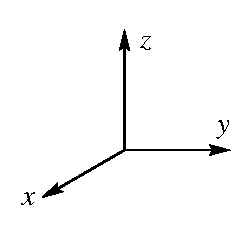
\includegraphics[scale=0.6]{figure/repere_orbitale.eps} & 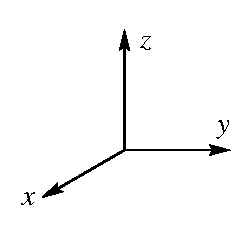
\includegraphics[scale=0.6]{figure/repere_orbitale.eps} & 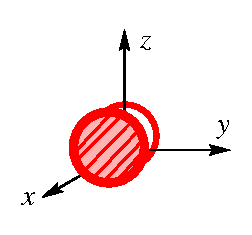
\includegraphics[scale=0.6]{figure/orbitale.eps} & 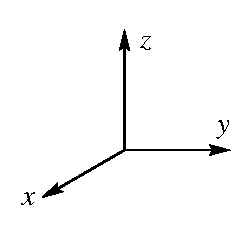
\includegraphics[scale=0.6]{figure/repere_orbitale.eps} & 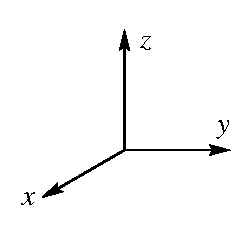
\includegraphics[scale=0.6]{figure/repere_orbitale.eps} \\
$1s$ & $2s$ & $2p_x$ & $2p_y$ & $2p_z$
\end{tabular}
\end{center}
%--------------------------------------------------------------------------
%\exo{\'Etude des \'el\'ements des 1$^\textrm{er}$ et 2$^\textrm{e}$ groupes}
%\begin{enumerate}[\bf 1)]
%\item Nommez les \'el\'ements alcalins.
%\item On donne la s\'erie des valeurs d'\'energies d'ionisation en kJ.mol$^{-1}$~: 375,6~; 402,9~; 418,7~; 495,7 et 520,1 pour ces \'el\'ements. Attribuez chaque valeur \`a un \'el\'ement, sachant qu'aucune valeur n'est donn\'ee pour le Francium. Expliquez la variation des \'energies d'ionisation dans la colonne.
%\item \'Ecrire la structure \'electronique \underline{de valence} des \'el\'ements du 2$^\textrm{e}$ groupe.
%\item Dites comment \'evoluent les grandeurs suivantes par rapport aux \'el\'ements alcalins~:
%\begin{enumerate}%[~~~-]
%\item degr\'e d'oxydation le plus souvent rencontr\'e,
%\item dimension,
%\item \'energie de premi\`ere ionisation.
%\end{enumerate}
%\end{enumerate}
%--------------------------------------------------------------------------
\exo{Configuration \'electronique et classification p\'eriodique}
\begin{enumerate}[\bf 1)]
\item Soit l'\'el\'ement $_{31}^{69}$Ga. \'Ecrire sa configuration \'electronique atomique.
Dans quel bloc de la classification p\'eriodique se trouve cet \'el\'ement~?
Sur quelle p\'eriode~?
Dans quelle colonne~?
\item M\^emes questions pour les \'el\'ements $_{~6}^{12}$C, $_{15}^{31}$P, $_{20}^{40}$Ca, 
$_{22}^{48}$Ti, $_{32}^{71}$Ge et $_{38}^{88}$Sr.
\item Comparez les rayons atomiques des \'el\'ements appartenant \`a une m\^eme p\'eriode/\`a une m\^eme colonne.
\end{enumerate}
{\bf Exercice supplémentaire}
\exo{Propri\'et\'es des \'el\'ements et classification p\'eriodique}
\begin{enumerate}[\bf 1)]
%\item \'Ecrire la structure \'electronique des ions suivants : I$^-$, Fe$^{2+}$, Cr$^{3+}$.
\item Classez les \'el\'ements suivants par ordre croissant de leur rayon atomique, puis par ordre croissant
de leur énergie de première ionisation :
\begin{enumerate}%[~~~-]
\item Rb, Li, Na, K
\item Cl, Na, P, S, Mg, Si, Al
\end{enumerate}
\item Commentez la variation de l'\'electron\'egativit\'e dans le tableau p\'eriodique. Classez les \'el\'ements suivants par ordre d\'ecroissant d'\'electron\'egativit\'e : K, F, Na, Cl, I.
\item Dites comment \'evoluent les grandeurs suivantes pour les alcalino terreux~:
\begin{enumerate}%[~~~-]
%\item degr\'e d'oxydation le plus souvent rencontr\'e,
\item rayon atomique,
\item \'energie de premi\`ere ionisation.
\end{enumerate}
\end{enumerate}
%

\titreTD{\thenumTD}{Mod\`ele de Slater}

\meth{Application du mod\`ele de Slater \`a l'h\'elium}
On se propose dans ce probl\`eme de d\'eterminer l'\'energie de premi\`ere ionisation de l'h\'elium \`a partir du mod\`ele de Slater.
\begin{enumerate}[\bf 1)]
\item Quelle est la valeur du num\'ero atomique $Z$ de l'atome d'h\'elium~?
\item Quelle est la structure \'electronique de cet \'el\'ement dans son \'etat fondamental~?
\item Donnez la valeur des nombres quantiques de chaque \'electron.
\item Sachant que l'effet d'\'ecran d'un \'electron 1$s$ sur un \'electron 1$s$ est d\'ecrit par la constante de Slater $\sigma_{1s}=0.30$, calculez la charge nucl\'eaire effective ressentie par un tel \'electron. 
\item En d\'eduire l'\'energie d'un \'electron de l'atome d'h\'elium.
\item En d\'eduire l'\'energie $E(\textrm{He})$ de l'atome d'h\'elium dans son \'etat fondamental.
\item Comment appelle-t-on un cation du type de He$^+$~?  En d\'eduire l'\'energie $E(\textrm{He}^+)$.
\item Montrez que l'\'energie de premi\`ere ionisation de l'h\'elium vaut $E_\textrm{ionis.}(\textrm{He})=24.2$~eV.
\item Quelle est la valeur minimale de la fr\'equence de la radiation que l'on doit utiliser pour ioniser 
une fois l'h\'elium~? 
\end{enumerate}
%--------------------------------------------------------------------------
\exo{Application du mod\`ele de Slater au magn\'esium}
\begin{enumerate}[\bf 1)]
\item Quelle est la configuration \'electronique du magn\'esium dans l'\'etat fondamental~?
\item D\'eterminez la charge nucl\'eaire effective puis l'\'energie de chaque \'electron.
\item \'Evaluez l'\'energie totale d'un atome de magn\'esium et d'un ion Mg$^+$.
\item En d\'eduire la valeur de l'\'energie de premi\`ere ionisation du magn\'esium.
\end{enumerate}
%--------------------------------------------------------------------------
\exo{Rayon atomique}
\begin{enumerate}[\bf 1)]
\item Donnez la configuration \'electronique des atomes de la deuxi\`eme p\'eriode du tableau p\'eriodique.
\item Compl\'etez le tableau ci-dessous. Les valeurs de $n$, $Z_{eff}$ et $r$ ne sont \`a calculer \textbf{que} pour 
la derni\`ere orbitale occup\'ee.

%\begin{tabular}{p{3cm}|c|c|c|c|c|c|c|c}
%\hline
%\'El\'ement (Z)                               & Li (3) & Be (4) & B (5) & C (6) & N (7) & O (8) & F (9) & Ne (10) \\
%\hline
%$n$ de la derni\`ere orbitale occup\'ee       &&&&&&&&\\
%$Z_{eff}$ de la derni\`ere orbitale occup\'ee & 1.3    & 1.95   &&&&&&\\
%$r$ de la derni\`ere orbitale occup\'ee       &        &        & 1.54 $a_0$ & 1.23 $a_0$ & 1.03 $a_0$ & 0.88 $a_0$& 0.77 $a_0$&\\
%\hline
%\end{tabular}

\vrule

\begin{tabular}{p{3cm}|c|c|c|c|c|c|c|c}
\hline
\textbf{\'El\'ement (Z)}                               & Li (3) & Be (4) & B (5) & C (6) & N (7) & O (8) & F (9) & Ne (10) \\
\hline
$n$        &&&&&&&&\\\hline
$Z_{eff}$  & 1.3    & 1.95   &&&&&&\\\hline
$r$        &        &        & 1.54 $a_0$ & 1.23 $a_0$ & 1.03 $a_0$ & 0.88 $a_0$& 0.77 $a_0$&\\
\hline
\end{tabular}

\vrule

\item Tracez les courbes donnant la variation de $r$ et de $Z_{eff}$ 
(de la derni\`ere orbitale occup\'ee) en fonction de Z. 
\end{enumerate}
%--------------------------------------------------------------------------
\exo{Potentiel d'ionisation}
\begin{enumerate}[\bf 1)]
\item Calculer les \'energies des atomes suivants~: C, He, Li, Ne, Al.
\item Calculer les \'energies de leurs monocations~: C$^+$, He$^+$, Li$^+$, Ne$^+$, Al$^+$.
%\marginpar{Paola: correzione PI He, Al}
\item Pour chaque esp\`ece, retouver les suivantes valeurs pour les potentiels de premi\`ere ionisation (en eV)~:
11,5 (C); 24,2 (He); 5,7 (Li); 16,0 (Ne); 10,8 (Al).
\end{enumerate}

\titreTD{\thenumTD}{Mod\`ele de Bohr --  Notions de spectroscopies}

%\exo{L'atome d'hydrog\`ene}
%
%Le mod\`ele de l'atome d'hydrog\`ene propos\'e par Rutherford et Perrin est le suivant~:
%un \'electron de charge $e$ tourne autour d'un proton en parcourant, d'un mouvement
%uniforme, une orbite circulaire de rayon $r$.
%
%\begin{enumerate}[\bf 1)]
%
%\item On se propose de trouver l'expression de l'\'energie totale de l'interaction \'electron/proton
%en employant les lois de la m\'ecanique classique et la loi de Coulomb.
%\begin{enumerate}
%\item Exprimer les forces en pr\'esence au niveau de l'\'electron, puis en faisant le bilan de ces forces
%\`a l'\'equilibre montrer que~:
%
%\begin{equation}
%\label{eq_bohr1}
%mv^2 = \frac{e^2}{4 \pi \varepsilon_0 r}
%\end{equation}
%
%\item En consid\'erant l'\'energie comme la somme des \'energies cin\'etique et potentielle,
%puis en se servant de l'\'equation~\ref{eq_bohr1}, montrer que~:
%
%\begin{equation}
%\label{eq_bohr2}
%E = \frac{-e^2}{8 \pi \varepsilon_0 r}
%\end{equation}
%
%\end{enumerate}
%
%\item En  posant l'hypoth\`ese de Bohr~:
%
%\begin{equation}
%\label{eq_bohr3}
%mvr = n\frac{h}{2\pi}
%\end{equation}
%
%\'etablir l'expression de $r$ dans l'atome d'hydrog\`ene, puis la nouvelle expression de l'\'energie.
%
%\item  Calculer le rayon de la premi\`ere orbite de Bohr (n=1) pour l'atome d'hydrog\`ene,
%en v\'erifiant l'\'equation aux dimensions.
%
%%\item Calculer la vitesse (en ms$^{-1}$) de l'\'electron sur la premi\`ere orbite de Bohr de l'atome
%%d'hydrog\`ene.
%\end{enumerate}


\exo{Spectroscopies d'absorption et d'emission: c'est lumineux.}
Pour attirer un partenaire sexuel, les vers luisant produisent une lumière verte.
Cette lumière est due à une réaction chimique:
\footnote{Bulletin de l'Académie Lorraine des Sciences 2005, 44 (1-4)}
il s’agit de l'oxydation d'une molécule organique, la luciférine qui s'oxyde sous l’effet de l’ATP
et d’ions magnésium, catalysée par une enzyme, la luciférase.
L’énergie biochimique se transforme en lumière.
\footnote{adapté de Alice Despinoy – http://lanaturedepres.fr}
%\begin{enumerate}[\bf 1)]
	%\item Est-ce un phénomène d'absorption ou d'emission?
	Est-ce un phénomène d'absorption ou d'emission?
%\end{enumerate}

\exo{Spectroscopies d'absorption et d'emission: Bon appétit bien sûr!}
Les cochenilles sont de charmants insectes d'environ 5mm.
Elles se défendent en sécrétant de l'acide carminique qui est utilisé depuis le Moyen Âge comme colorant
rouge comme son nom l'indique.
Actuellement, ce colorant est utilisé comme colorant alimentaire (sous le nom de E120 dans des viandes, sirops, biscuits, bonbons, etc.), cosmétique (où il prend le nom CI 75470 dans des dentifrices, rouges à levre, etc) ou autre.

%\begin{enumerate}[\bf 1)]
	%\item Lorsque l'on regarde un verre de grenadine, il paraît rouge.
	%	Est-ce un phénomène d'absorption ou d'emission?
	      Lorsque l'on regarde un verre de grenadine, il paraît rouge.
		Est-ce un phénomène d'absorption ou d'emission?
%	\item Les états fondamentaux et excités impliqués sont-ils atomiques ou moléculaires?
%\end{enumerate}

\exo{Notions de spectroscopies}

\begin{enumerate}[\bf 1)]
\item On consid\`ere l'atome d'hydrog\`ene (Z=1) et d'h\'elium (Z=2).
\begin{enumerate}
\item Expliquer pourquoi He$^+$ est un hydrog\'eno\"ide.
%\item Calculer en eV les potentiels d'ionisations pour H et He$^+$.
\item Calculer les \'energies des diff\'erents niveaux quantiques ($n$ = 2 \`a 6) pour l'hydrog\`ene et He$^+$
en eV et en Joules. Tracer ces niveaux sous formes de diagrammes en eV.
\end{enumerate}

\item Lorsque l'\'electron se d\'esexcite (de $n_i$ \`a $n_f < n_i$) il \'emet de la lumi\`ere avec
une \'energie correspondant exactement \`a la diff\'erence d'\'energie entre les niveaux $n_f$ et $n_i$.
On rappelle que $E=hc/\lambda$. Le spectre d'\'emission de la s\'erie de Balmer pour l'hydrog\`ene
a \'et\'e le premier observ\'e car il est dans le domaine spectral visible (400 \`a 800 nm).
\begin{enumerate}
\item Montrer que la s\'erie de Lyman ($n_f =1$) n'est pas dans le domaine visible.
\item A quelle \'energie (en eV) correspond la longueur d'onde 400 nm ?
\item A quelle \'energie (en eV) correspond la longueur d'onde 800 nm ?
\item Sur la base de l'exercice 1c), donner pour He$^+$ des valeurs de $n_i$ et de $n_f$ pour
que la transition se produise dans le visible, commenter.
\end{enumerate}

\item On considère à présent l’atome d’hydrogène dans l’état électronique excité caractérisé par
n$_2$ = 3.
\begin{itemize}
\item Quels sont les chemins de désexcitation possibles pour que l’atome arrive à son niveau
fondamental n 1 = 1 ?
\item Combien de raies d’émission observe-t-on ? Lesquelles ?
\item Mêmes questions si l’atome d’hydrogène est dans l’état excité caractérisé par n$_2$ = 4.
\item L’atome H étant toujours dans l’état excité n$_2$ = 4, on suppose qu’au cours de la
désexcitation, la population se répartit de façon égale entre les différents niveaux
possibles. Par exemple si l’on a 100 atomes excités au départ, et s’il y a 3 niveaux
accessibles lorsqu’un électron fait une transition vers un niveau inférieur, alors 33
électrons feront la transition vers chacun des niveaux possibles. Et le même
raisonnement se poursuit pour les transitions qui finissent par ramener les atomes à
leur niveau fondamental. Combien d’atomes feront alors la transition 2$\rightarrow$1 sachant que
l’on a 100 atomes excités au départ ?
\end{itemize}


%\item Bien avant la th\'eorie de Bohr, Balmer et Rydberg ont \'etabli la relation empirique
%permettant de calculer les longueurs d'onde des raies d'\'emission du spectre de l'atome d'hydrog\`ene~:
%\begin{equation}
%\label{eq_ryd}
%\frac{1}{\lambda} = R_H \left( \frac{1}{n^2_f} - \frac{1}{n^2_i} \right)
%\end{equation}
%dans laquelle $n_f$ et $n_i$ sont des entiers et $R_H$ une constante, appel\'ee constante de Rydberg.
%Trouver que $R_H = 1,097.10^7 m^{-1}$.
%%Calculer la valeur de la constante de Rydberg.
\end{enumerate}

%{\textcolor{red} Donn\'ees}

%\vspace{1cm}
%\small{
%\begin{tabular}{lll}
%\multicolumn{3}{l}{\bf Donn\'ees}\\
%$c$              & (vitesse de la lumi\`ere) & = 3*108 m.s$^{-1}$\\
%$h$              & (constante de Planck)     & = 6.624*10$^{-34}$ J.s\\
%$m$              & (masse de l'\'electron)   & = 9.10*10$^{-31}$ kg\\
%$e$              & (charge \'el\'ementaire)  & = 1.602*10$^{-19}$ C\\
%$\varepsilon_0$  & (permitivit\'e du vide)   & = 8.854*10$^{-12}$ C$^2$.J$^{-1}$.m$^{-1}$\\
%\multicolumn{3}{l}{1 J = 1 m$^2$kg.s$^{-2}$}\\
%\multicolumn{3}{l}{1 J = 6.241*10$^{18}$ eV}\\
%\end{tabular}
%}
\exo{Spectroscopies d'absorption et d'emission: Trop chaud!}
Le Soleil emet une lumière à large spectre, c'est-à-dire que
l'on peut faire l'hypothèse que toutes les longueurs d'onde sont émise
avec une égale intensité.
Or, l'analyse du spectre de la lumière solaire à la surface de la Terre met en évidence
des longueurs d'onde manquantes que l'on appelle raies de Fraunhofer :\\
\begin{pspicture}(\textwidth,5cm)
%	\put(0,5){\psspectrum[lines={299,302,336,358,382,393,396,410,430,430,434,438,466,486,495,516,516,516,517,518,527,546,587,588,589,627,656,686,759,822,898},lwidth=0.04,axe,absorption,brightness=1.0](\linewidth,2.5)}
%	\put(0,2){\psspectrum[lines={410,434,486,656},lwidth=0.04,axe,absorption,brightness=1.0](\linewidth,2.5)}
	\put(0,2){\psspectrum[lines={299,302,336,358,382,393,396,410,430,430,434,438,466,486,495,516,516,516,517,518,527,546,587,588,589,627,656,686,759,822,898},lwidth=0.04,axe,Dl=50,absorption,brightness=1.0](\linewidth,2.5)}
%	\put(0,2){\psspectrum[lines={410,434,486,656},lwidth=0.04,axe,absorption,brightness=1.0](\linewidth,2.5)}
	\put(3,1){\textbf{Domaine visible - Longueur d'onde (nm)}}
\end{pspicture}
\begin{enumerate}[\bf 1)]
	\item Faire un schema qui fasse apparaître le Soleil, la Terre entourée de son atmosphère
		ainsi que le rayonnement solaire qui arrive sur Terre.
	\item Ces raies sont-elles dues à des phénomènes d'absorption ou d'emission?
		Expliquer à l'aide d'un schema.
	\item On note particulièrement que les 4 longueurs d'ondes suivantes sont manquantes:
		656 nm, 486 nm, 434 nm et 410 nm. Pouvez-vous proposer une explication?
%	\item À quel endroit les phénomènes responsables des raies de Fraunhofer ont-ils lieu? Est-ce
%		à la surface du Soleil, entre le Soleil et la Terre, dans l'atmosphère, à la surface
%		de la Terre?

\end{enumerate}



%%--------------------------------------------------------------------
\titreTD{\thenumTD}{VSEPR et introduction \`a l'hybridation}

\exo{Mol\'ecules simples}

Dans un tableau, pour chaque mol\'ecule de l'ensemble I, pr\'ecisez pour chaque atome diff\'erent de H~:

\begin{itemize}
\item l'expression VSEPR AX$_n$E$_m$;
\item la figure de r\'epulsion;
\item la g\'eom\'etrie r\'eelle;
\item le type d'hybridation.
\end{itemize}


\exo{Mol\'ecules organiques simples}

Pour les mol\'ecules de l'ensemble II, \'etablir le type d'hybridation de chaque atome de carbone.

\exo{R\'ecapitulatif}

Compl\'eter le tableau suivant en indiquant l'expression VSEPR AX$_n$E$_m$, le type 
d'hybridation et le degr\'e d'oxydation des atomes de carbone en gras.

\clearpage

%\rotatebox{90}{%
%\parbox{15cm}{
\begin{landscape}
\begin{center}
%\begin{tabular*}{1.0\textheight}{@{\extracolsep{\fill}}rlllll}
\renewcommand{\arraystretch}{4}
\begin{tabular*}{20cm}{@{\extracolsep{\fill}}|r|c|c|c|c|c|}
\hline
                                       & \multicolumn{5}{c|}{\textbf{R$^\mathbf{1}$}} \\
\hline
                                       &CH$_3$ & OH & OCH$_3$ & NH$_2$ & NHCH$_3$ \\
\hline
\textbf{C}H$_3$-R$^1$                  &       &    &         &        & \\\hline 
%
CH$_3$-\textbf{C}H$_2$-R$^1$           &&&&&\\\hline

\begin{pspicture}(2.3,1)                     
%\showgrid
\put(0.0,0.6){CH$_3$}\psline(0.8,0.6)(0.97,0.4)
\put(1.0,0.3){\textbf{C}H-R$^1$}
\put(0.0,0.0){CH$_3$}\psline(0.8,0.15)(0.97,0.4)
\end{pspicture}                        &&&&&\\\hline
%
%\begin{pspicture}(1.9,1.5)                     
%%\showgrid
%\put(0.0,0.6){CH$_3$-\textbf{C}-R$^1$}
%\put(0.85,0.0){CH$_3$}\psline(1.05,0.35)(1.05,0.57)
%\put(0.85,1.15){CH$_3$}\psline(1.05,0.90)(1.05,1.12)
%\end{pspicture}                        &&&&&\\\hline
%
CH$_3$-\textbf{C}(O)-R$^1$ &&&&&\\\hline
%H\textbf{C}O-R$^1$       &&&&&\\\hline
R$^1$-\textbf{C}HO         &&&&&\\\hline
\end{tabular*}
\end{center}
\end{landscape}
%}
%}

%\titreTD{\thenumTD}{Les orbitales hybrides}

\exo{Les diff\'erents types d'hybridation}

Soit les mol\'ecules ci-apr\`es et leur figure de r\'epulsion (FR) selon VSEPR.

\begin{enumerate}[\bf 1)]
\item Quel type d'hybridation pour le \textbf{Si} dans SiH$_4$, pour le \textbf{C} et le \textbf{O} dans le formol 
(H$_2$CO) et pour le \textbf{C} et le \textbf{N} dans l'acide cyanhydrique (HCN) permet d'expliquer les figures de 
r\'epulsion bas\'ees sur la th\'eorie VSEPR~?
\begin{figure}[!h]
\begin{center}
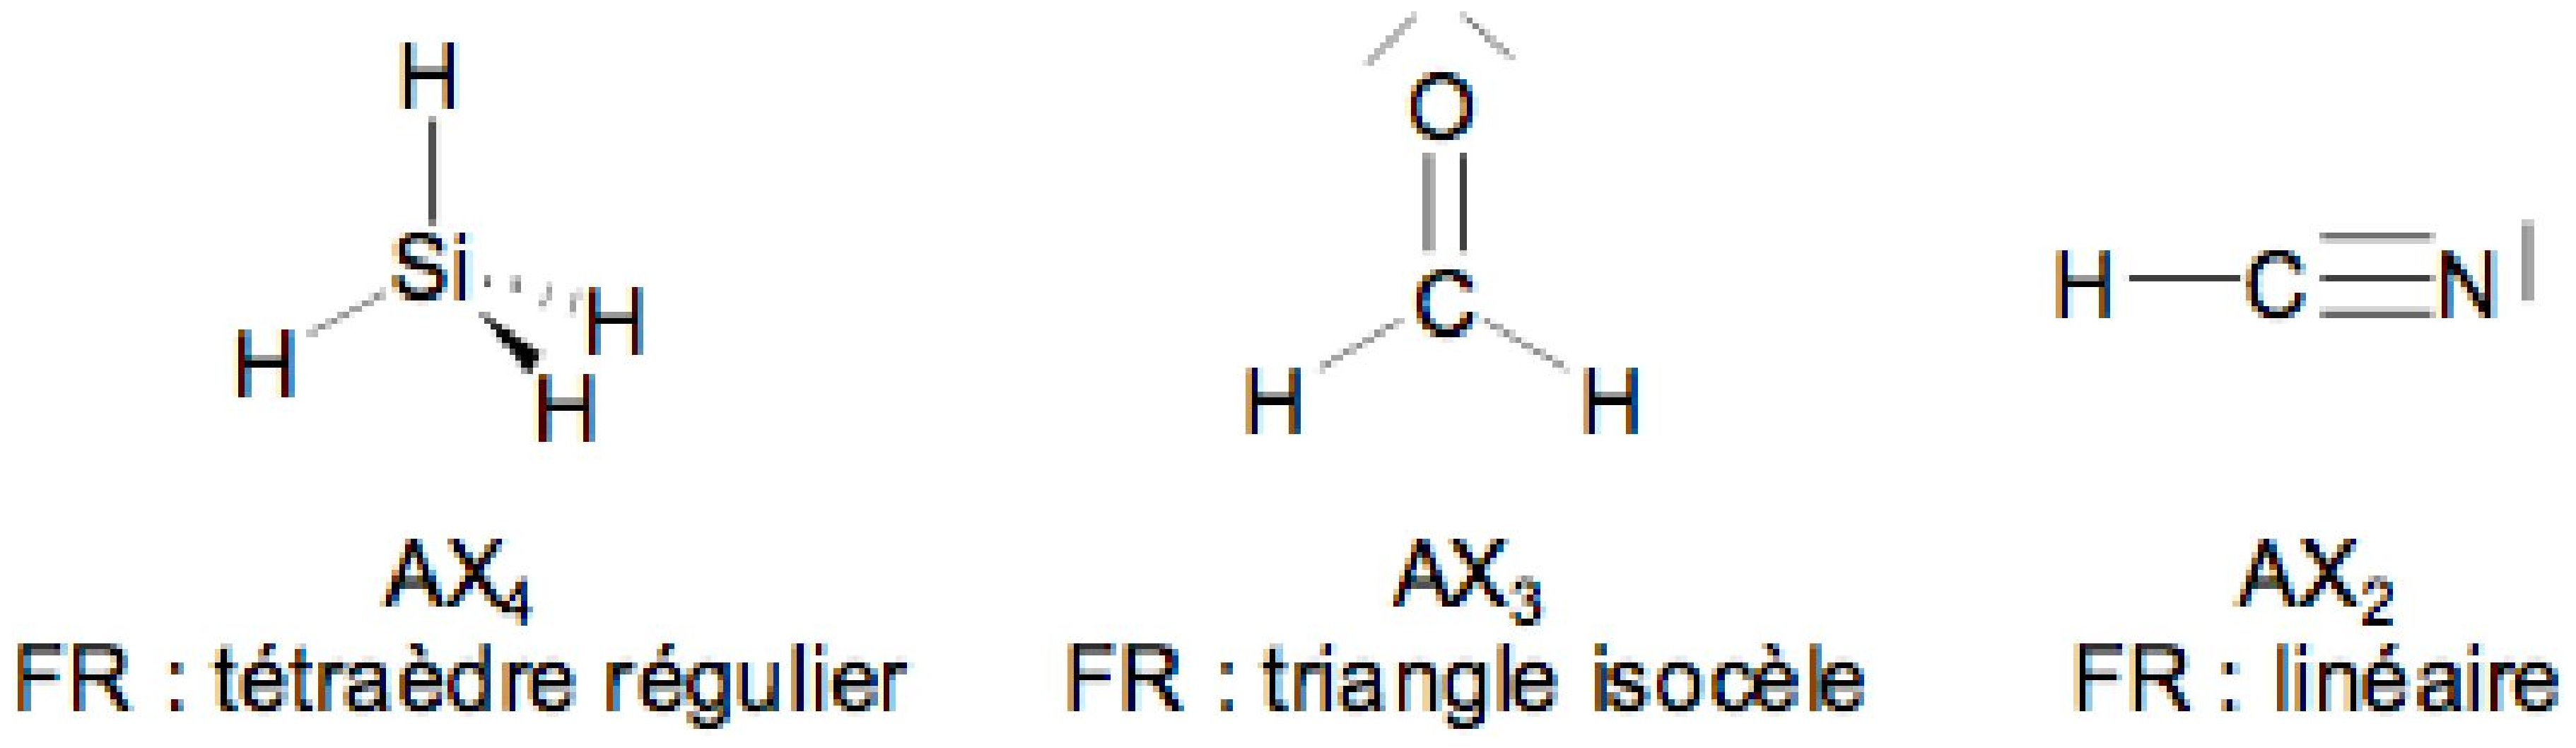
\includegraphics[scale=0.17]{figure/vsepr2.eps}
\end{center}
\end{figure}

\item Dessinez les trois mol\'ecules en faisant appara\^itre les orbitales atomiques hybrides et non hybrides des 
diffi\'erents atomes.
\item Pour chacune des mol\'ecules, donnez les diff\'erents types de liaisons ou 
orbitales mol\'eculaires form\'ees ($\sigma$ ou $\pi$).
\end{enumerate}

\textit{La r\'edaction de l'exercice pourra se faire selon l'exemple donn\'e ci-dessous :}\\
Mol\'ecule d'\'ethyl\`ene~:

%
\begin{figure}[!h]
\begin{center}
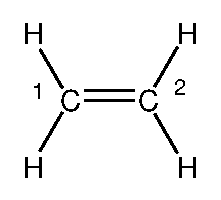
\includegraphics[height=2.0cm]{figure/vsepr3.eps}
\end{center}
\end{figure}
%

Ce carbone (1) est entour\'e de trois liaisons selon la th\'eorie VSEPR~: 2 simples, une double. Il est donc de type AX$_3$. 
Couche de valence du carbone : $2s^2 2p^2$.
%
\begin{figure}[!h]
\begin{center}
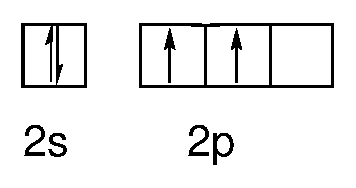
\includegraphics[height=1.5cm]{figure/vsepr4.eps}
\end{center}
\end{figure}
%

Pour cr\'eer \textbf{3} liaisons autour du carbone il faut \textbf{3} orbitales hybrides~:\\
\textbf{1} orbitale atomique (OA) $s$ + \textbf{2} OA $p$ = \textbf{3} OA hybrides de type $sp^2$.\\
Conclusion, une fois hybrid\'e, le carbone poss\`ede 3 OA hybrides de type $sp^2$ et il lui reste donc une orbitale $p$
non transform\'ee. On peut alors r\'epartir les 4 \'electrons dans ces 4 orbitales de fa\c{c}on \`a former 
les liaisons avec les voisins.
\begin{figure}[!h]
\begin{center}
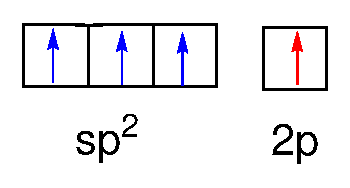
\includegraphics[height=1.5cm]{figure/vsepr5.eps}
\end{center}
\end{figure}

\clearpage

\textbf{Repr\'esentation}:
OA hybride de type sp$^2$~:     OA de type $p$ restante (remarque: on obtient le mi\^eme r\'esultat pour le carbone 2)
\begin{figure}[!h]
\begin{center}
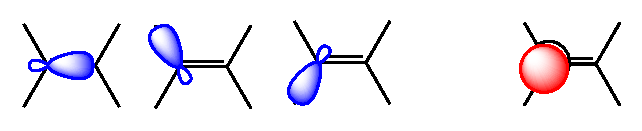
\includegraphics[height=1.5cm]{figure/vsepr6.eps}
\end{center}
\end{figure}

\textbf{Repr\'esentation} du carbone 1~: 
%3 OA hybrides de type $sp^2$ et une OA de type $p$ 
%(remarque: on obtient le mi\^eme r\'esultat pour le carbone 2) - 
Approche des hydrog\`enes -- Visualisation des diff\'erentes 
liaisons ou orbitales moli\'eculaires (OM) form\'ees.
\begin{figure}[!h]
\begin{center}
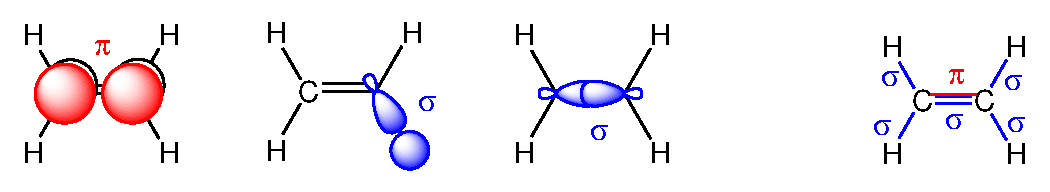
\includegraphics[height=2.5cm]{figure/vsepr7.eps}
\end{center}
\end{figure}


\exo{Hybridation}
\begin{enumerate}[\bf 1)]
\item Exemple de H-Be-H (mol\'ecule lin\'eaire, $sp$)\\
Une orbitale hybride $sp$ se construit en combinant une orbitale $s$ et une orbitale $p$ d'un m\^eme atome (ici Be). 
Pour un tel couple, on peut former 2 hybrides $sp$.
\begin{enumerate}
\item Repr\'esentez sch\'ematiquement chacune de ces 2 hybrides (un dessin par orbitale).
\item Combien d'orbitales $p$ restent pures sur Be~?
Les dessiner (un dessin par orbitale).
\end{enumerate}
\item Exemple de CH$_3^+$ (cation triangulaire, $sp^2$)\\
Les orbitales hybrides $sp^2$ sont construites par la combinaison d'une orbitale $s$ et de 2 orbitales $p$ d'un m\^eme atome (ici C).
\begin{enumerate}
\item Dessinez chacune de ces 3 hybrides (un dessin par orbitale).
\item Combien d'orbitales $p$ restent pures sur C~?
Les dessiner (un dessin par orbitale).
\end{enumerate}
\end{enumerate}

%\titreTD{\thenumTD}{M\'esom\'erie}

\exo{Formes limites}

Donner la structure de Lewis et la g\'eom\'etrie de l'ion carbonate CO$_3^{2-}$. 
L'exp\'erience montre que pour cet ion les liasons C-O sont \'equivalentes (0.129~nm).
Justifier ce r\'esultat.

\exo{Effets +M et -M sur des syst\`emes simples}

En justifiant par l'hybridation des atomes ($sp$, $sp^2$, $sp^3$), identifiez les sites donneurs et 
accepteurs de m\'esom\'erie (+M et $-$M) des structures de Lewis suivantes, et proposez un sch\'ema 
envisageable de mobilit\'e \'electronique (avec 1 ou 2 fl\`eches).

\begin{center}
\begin{tabular}{ccccc}
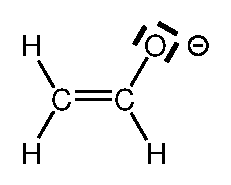
\includegraphics[scale=0.7]{figure/meso1.eps} & \, & 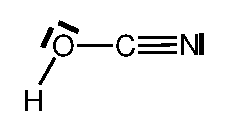
\includegraphics[scale=0.7]{figure/meso2.eps} & \, &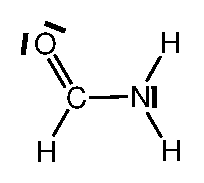
\includegraphics[scale=0.7]{figure/meso3.eps} \\
1& &2& &3\\[0.2cm]
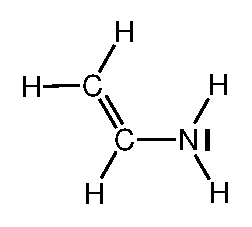
\includegraphics[scale=0.7]{figure/meso4.eps} &    &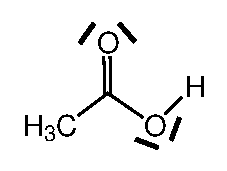
\includegraphics[scale=0.7]{figure/meso5.eps} &  &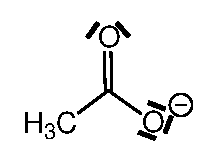
\includegraphics[scale=0.7]{figure/meso6.eps} \\
4& &5&  &6\\
\end{tabular}
\end{center}

\exo{Cas r\'eels}
\'Etablir la structure de Lewis des mol\'ecules suivantes, et donnez leurs formes m\'esom\`eres 
les plus probables selon les r\`egles usuelles (respect de l'octet, limitation de la s\'eparation de charge, etc...).

%\begin{figure}[!h]
\begin{center}
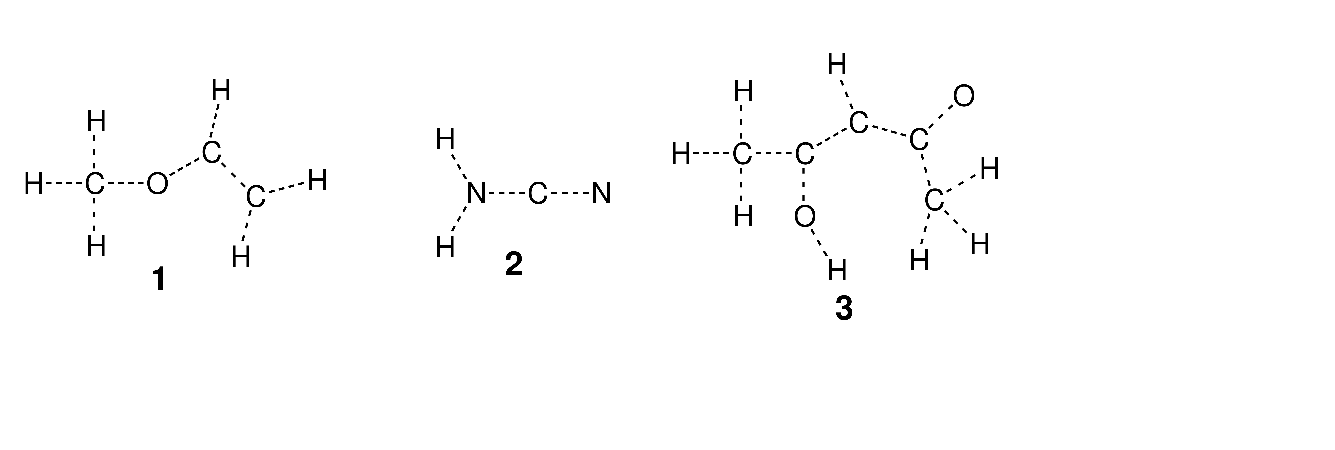
\includegraphics[scale=0.77]{figure/lewis4.eps}
\end{center}
%\end{figure}

\vrule

\clearpage

\exo{M\'esom\'erie}

Proposez un sch\'ema envisageable de mobilit\'e \'electronique (avec 1 ou 2 fl\`eches) pour
les mol\'ecules suivantes~:

\begin{center}
\begin{tabular}{ccc}
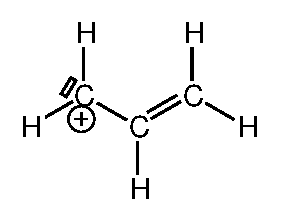
\includegraphics[scale=0.7]{figure/ex2meso1.eps} & \, & 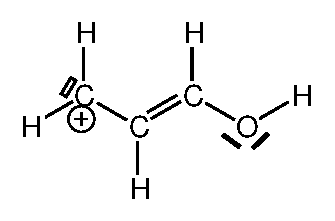
\includegraphics[scale=0.7]{figure/ex2meso2.eps} \\
1&&2\\[0.2cm]
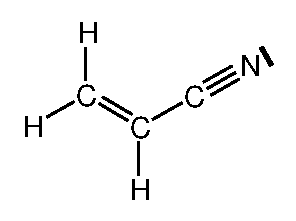
\includegraphics[scale=0.7]{figure/ex2meso3.eps} & \, & 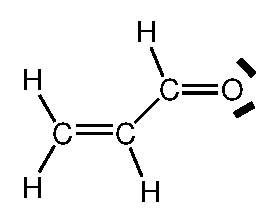
\includegraphics[scale=0.7]{figure/acrolein.eps} \\
3&&4\\
\end{tabular}
\end{center}




\titreTD{\thenumTD}{Recouvrements entre Orbitales Atomiques}

%##########################################################################
% NOTION DE RECOUVREMENT 
%##########################################################################

\textit{Pour se pr\'eparer \`a ces exercices, on pourra rappeler les sch\'emas des orbitales s, $p_x$, $p_y$, $p_z$ selon un rep\`ere impos\'e}.

\begin{center}
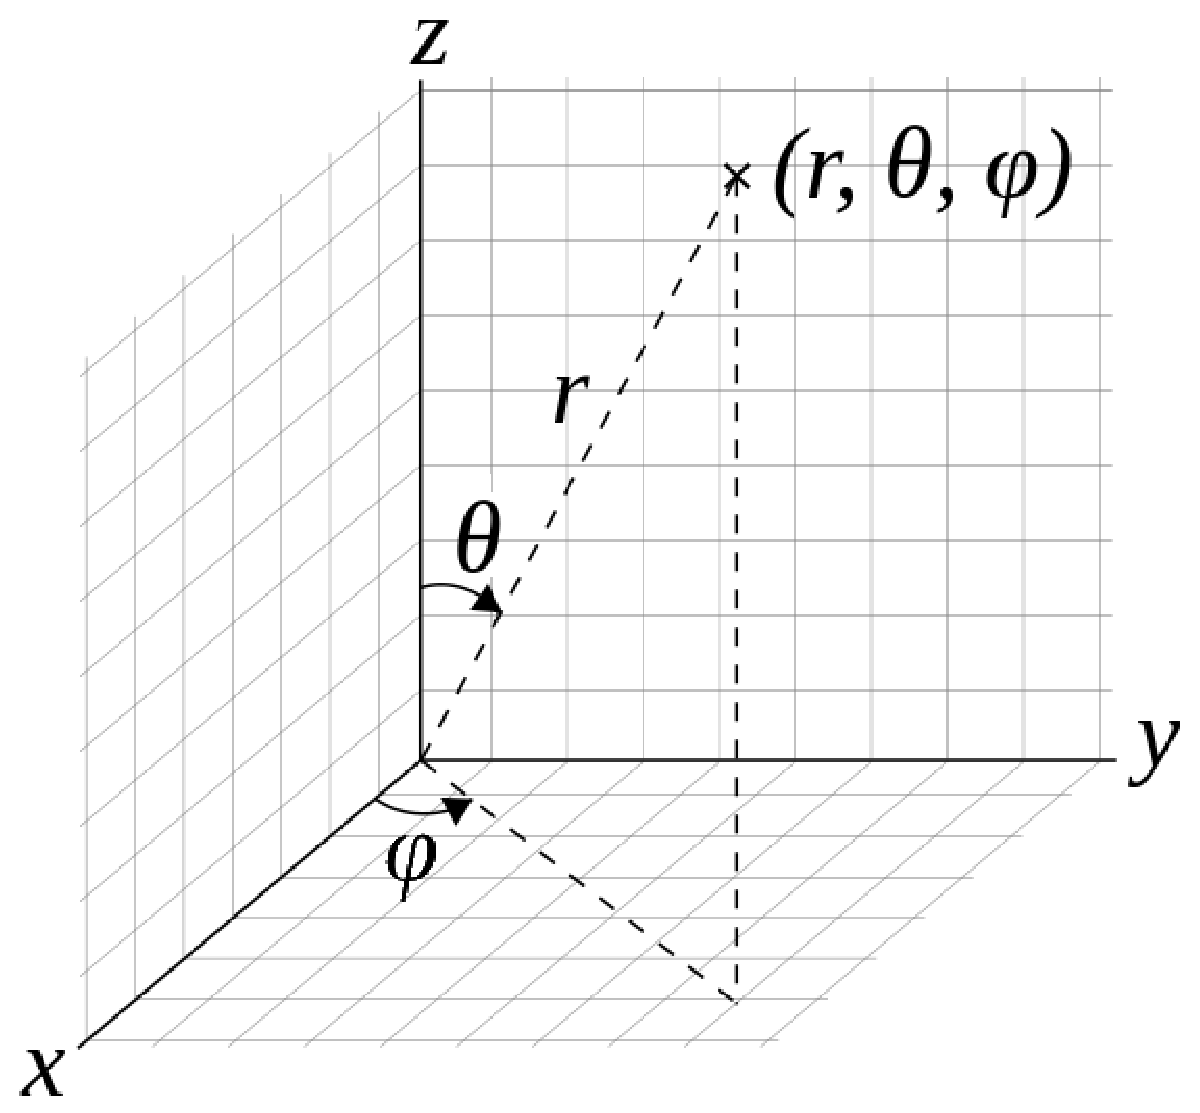
\includegraphics[height=9.5cm]{figure/spheriques_ok.eps}\\
\end{center}

\exo{D\'efinition}
\begin{enumerate}[\bf 1)]
\item   Rappelez l'expression du recouvrement $S_{ab}$, entre une orbitale $ \chi_a(x,y,z)$, et
$\chi_b(x,y,z)$.
\item  Que vaut exactement cette int\'egrale si $ \chi_a(x,y,z)=\chi_b(x,y,z)=\chi(x,y,z)$.
\item    Montrez graphiquement que les orbitales $2s_A$ et $2p_{z_{A}}$ (centr\'ee sur le m\^eme atome A), ont un recouvrement nul. Expliquez.
%\item    A quoi correspond la combinaison  $2s_A+2p_{z_{A}}$~? 
\end{enumerate} %\exo{Variation du Recouvrement avec la distance}
\exo{Recouvrement d'orbitales atomiques}
\label{exo_s}
Dans une mol\'ecule A$-$B, on \'etudie le recouvrement entre 2 orbitales atomiques, l'une centr\'ee sur un atome A, l'autre sur  B. Pour l'ensemble de cet exercice, les axes sont d\'efinis selon la figure du rep\`ere ci-dessous (l'axe internucl\'eaire d\'efinit l'axe Oz, et $x$ est dans le plan de la feuille, vers le haut). 
\\

Pour chaque cas propos\'e,

\begin{minipage}[c]{0.8\linewidth}
\begin{enumerate}[(i)] 
\item dessinez les orbitales en pr\'esence
\item indiquez la nature du recouvrement : $\sigma$, $\pi$ ou nul 
\item  pr\'ecisez s'il s'agit d'un recouvrement positif, n\'egatif ou nul
\end{enumerate} 
\end{minipage}
\begin{minipage}[l]{0.1\linewidth}     
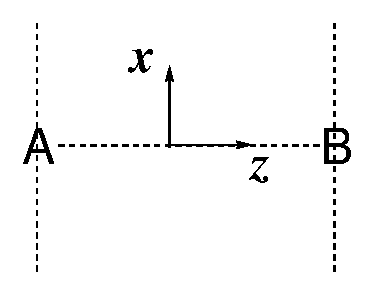
\includegraphics[scale=0.4]{figure/AB_repere.eps}\\   
Rep\`ere
\end{minipage}

\vspace{0.3cm}

\begin{minipage}[c]{0.5\linewidth}
\begin{enumerate}[\bf 1)]
\item $+2p_{x\textsc{a}}\ \, |+\,2p_{x\textsc{b}}$ 
\item $+2p_{z\textsc{a}}\ \, |-\,2p_{z\textsc{b}}$ 
\item $\ \, +2s_\textsc{a}\ \, |+\,2s_\textsc{b}$ 
\item $\ \, +2s_\textsc{a}\ \, |+\,2p_{z\textsc{b}}$ 
\item $+2p_{x\textsc{a}}\ \, |+\,2s_\textsc{b}$ 
%\item $+3p_{y\textsc{a}}\ \, |-\,3p_{y\textsc{b}}$
%\item $-3p_{x\textsc{a}}\ \, |-\,3s_\textsc{b}$
%\item $-2p_{x\textsc{a}}\ \, |-\,3p_{x\textsc{b}}$
\end{enumerate} 
\end{minipage} \hfill
\begin{minipage}[c]{0.5\linewidth}
 \textbf{Exemple :}  $+2s_\textsc{a}\ |-\,2s_\textsc{b}$
\begin{enumerate}[~~(i)] 
\item    Dessin~:\\[-0.3cm] 

   \  \  \  \  \   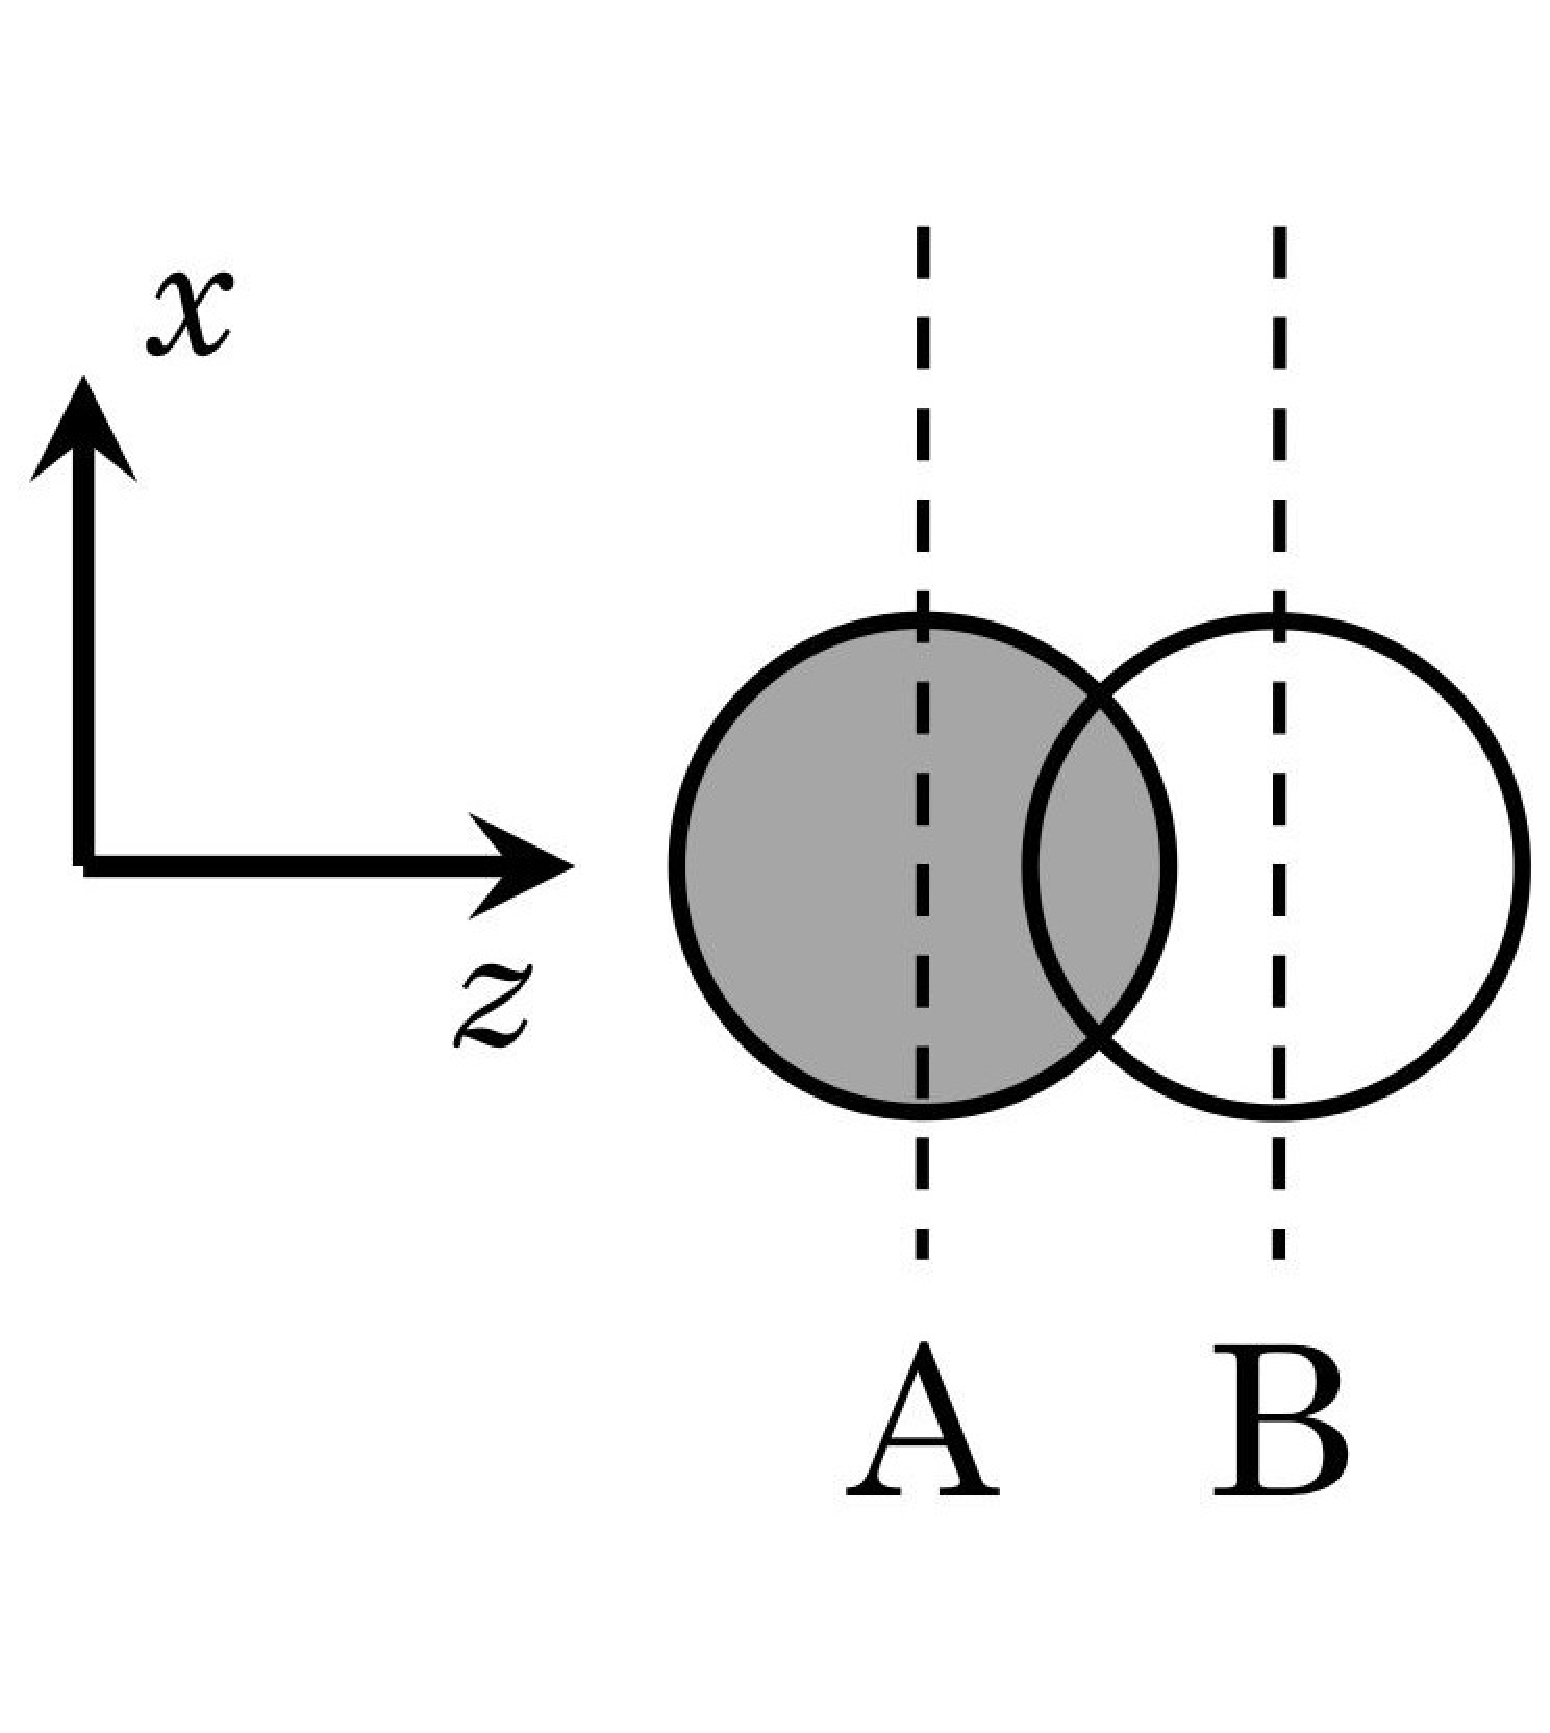
\includegraphics[scale=0.09]{figure/interactionOA.eps}
\item       Recouvrement axial, donc $\sigma$
\item       Recouvrement <0 car de phase $\neq $
\end{enumerate} 
\end{minipage}

%--------------------------------------------------------------------------
\meth{Évolution du recouvrement en fonction de la distance entre deux orbitales}
On consid\`ere une orbitale p$_z$ et une orbitale s qui s'approchent l'une de l'autre.
Dessiner l'allure de l'\'evolution du recouvrement entre elles.\\
\textsl{%
Le recouvrement entre deux orbitales $\phi_a$ et $\phi_b$ est donné par la formule~:
\begin{align*}
S = \int \phi_a \phi_b^* dV
\end{align*}
On peut voir cette intégrale comme une somme sur tout l'espace d'éléments infiniments
petits constitués du produit de ces deux orbitales.
Dans une zone de l'espace où les deux orbitales sont du même signe (même couleur)
le produit est positif.
À l'inverse, si les deux orbitales sont de signes (couleurs) opposés le produit est négatif.
Si la zone où le produit est positif est plus grande que celle où le produit est négatif,
le recouvrement est positif.
Dans les cas où ces deux zones ont exactement la même taille, le recouvrement est nul.
Sinon, il est négatif.
%
De manière à avoir une idée de la forme de la courbe qui donne le recouvrement en fonction
de la distance entre les orbitales, nous allons considérer plusieurs situations dans le tableau suivant~:\\
\rotatebox{90}{%
\begin{tabular}{|p{2cm}|p{4cm}|p{7cm}|p{3cm}|}\hline
Distance & Schema & Commentaire & Recouvrement\\\hline
$+\infty$                        & \raisebox{-1cm}{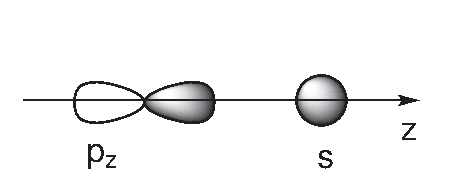
\includegraphics[width=4cm]{figure/ovl01.eps}} & Les orbitales sont sans interaction. & nul \\\hline
positive et grande               & \raisebox{-1cm}{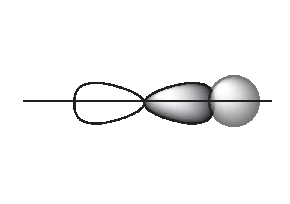
\includegraphics[width=3cm]{figure/ovl02.eps}} & Les orbitales interagissent faiblement. Dans cette zone elles sont toutes les deux du même signe (colorées). & petite valeur positive \\\hline
proche de la distance de liaison & \raisebox{-1cm}{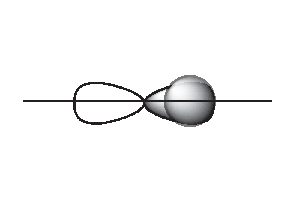
\includegraphics[width=3cm]{figure/ovl03.eps}} & Les orbitales se recouvrent largement: le recouvrement atteint sa valeur maximale.                           & positif et maximum    \\\hline
positive et courte               & \raisebox{-1cm}{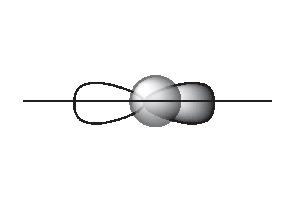
\includegraphics[width=3cm]{figure/ovl04.eps}} & Une partie des orbitales se recouvre avec un signe opposé (blanc et coloré) ce qui diminue le recouvrement.& petite valeur positive \\\hline
nulle                            & \raisebox{-1cm}{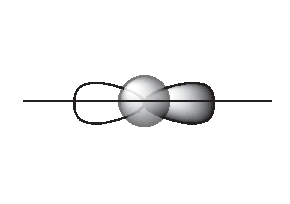
\includegraphics[width=3cm]{figure/ovl05.eps}} & La partie positive du recouvrement (lorsque les orbitales sont du même signe) est égale en valeur absolue à sa partie négative. & nul \\\hline
négative et courte               & \raisebox{-1cm}{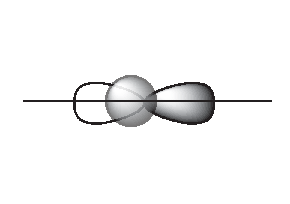
\includegraphics[width=3cm]{figure/ovl06.eps}} & Une partie des orbitales se recouvre avec un même signe ce qui diminue la valeur absolu du recouvrement.& petite valeur négative \\\hline
\end{tabular}
}
On obtient alors le graphe suivant~:\\
\begin{center}
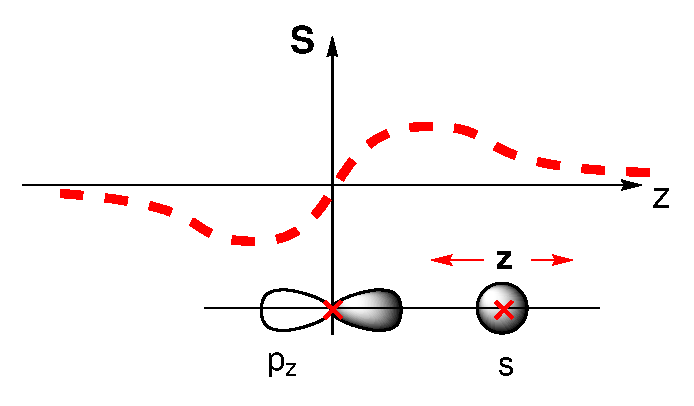
\includegraphics[width=8.0cm]{figure/exempl_recou_zs.eps}
\end{center}
}

\exo{Recouvrement entre orbitales}

Les dessins des orbitales donnent la forme g\'en\'erale du volume o\`u l'\'electron
a le plus de chance de se trouver. M\^eme quand ces orbitales ne se touchent pas
graphiquement, on a un recouvrement.

On consid\`ere deux orbitales qui s'approchent l'une de l'autre.
Dessiner l'allure de l'\'evolution du recouvrement entre les diff\'erentes orbitales
pour $z \in ]-\infty;+\infty[$.

%%FIGURE
\vspace{-0.3cm}
\begin{center}
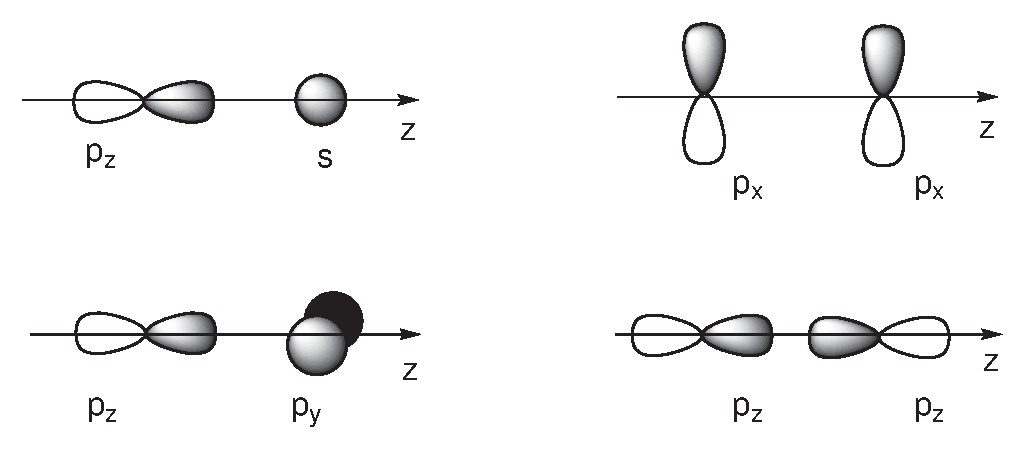
\includegraphics[width=8.0cm]{figure/overl1.eps}
\end{center}

\exo{Matrice de recouvrement}

Dans cet exercice le rep\`ere est defini de la mani\`ere suivante~:

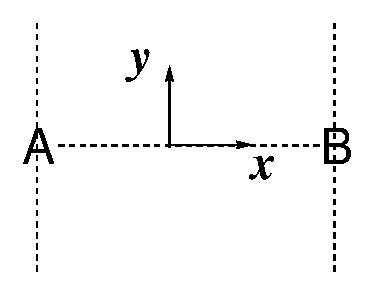
\includegraphics[width=2cm]{figure/AB_repere_yx.eps}

Pour deux atomes, A et B, s\'epar\'es d'une distance de liaison 
(environ 1.0-2.0~\AA), remplissez le tableau suivant avec les valeurs 0, 1 et $+$ ou $-$
selon la signe du recouvrement~:
%\begin{enumerate}
%\item $\chi_i = 1s_\textsc{a}$ et $\chi_j = 1s_\textsc{b}$~;
%\item $\chi_i = 2s_\textsc{a}$ et $\chi_j = 2s_\textsc{b}$~;
%\item $\chi_i = 2s_\textsc{a}$ et $\chi_j = 2p_{x\textsc{b}}$~;
%\end{enumerate}
%
%\item Remplissez le tableau suivant~:

\begin{tabular}{|c||c|c|c|c|c|}
\hline
                   & $2s_\textsc{a}$ & $2s_\textsc{b}$ & $2p_{x\textsc{b}}$ & $2p_{y\textsc{b}}$ & $2p_{z\textsc{b}}$ \\
\hline\hline
$2s_\textsc{a}$     & 1 & $+$ & $-$ & 0 & 0 \\ \hline
$2s_\textsc{b}$     &&&&& \\ \hline
$2p_{x\textsc{b}}$  &&&&& \\ \hline
$2p_{y\textsc{b}}$  &&&&& \\ \hline
$2p_{z\textsc{b}}$  &&&&& \\ \hline
\end{tabular}

\titreTD{\thenumTD}{Orbitales Mol\'eculaire, combinaison d'Orbitales Atomiques}

\parbox{0.5\textwidth}{\textit{Dans une mol\'ecule A$-$B, l'axe internucl\'eaire 
d\'efinit l'axe $Oz$, selon la figure du rep\`ere~:}}
\parbox{0.5\textwidth}{\centerline{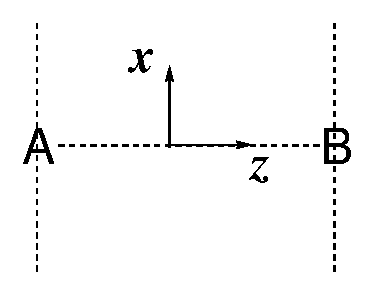
\includegraphics[scale=0.4]{figure/AB_repere.eps}}}

\exo{Principe de construction des diagrammes d'OM}
On consid\`ere l'interaction entre orbitales atomiques de deux atomes (A) et (B) formant une mol\'ecule A$-$B.
\begin{enumerate}[~~I.]
\item  $(1s_{A})$   et $(1s_{B})$ 
\item  $(2p_{x_A}, 2p_{z_A})$   et $(2p_{x_B},2p_{z_B})$ 
\item  $(2s_{A},2p_{x_A}, 2p_{y_A})$ et $(2s_{B},2p_{x_B},2p_{y_B})$
%\item   $(2s_{A}, 3d_{z^2\textsc{A}})$   et $(2s_{B},3d_{z^2\textsc{B}})$ 
\end{enumerate}
Pour chacun de ces  syst\`emes  ($\textsc{I}$, $\textsc{II}$ et $\textsc{III}$), 
repr\'esentez sur un diagramme d'\'energie le r\'esultat de l'interaction entre paires d'OA. 
Le cas \'ech\'eant, justifiez la d\'eg\'en\'erescence de certaines  OM. 
Pr\'ecisez pour chaque orbitale si elle est de type $\sigma$ ou $\pi$ et, si elle est  antiliante, 
indiquez le par une * (exemple $\sigma_1^*$).\\

\textit{On supposera que les OA non d\'eg\'en\'er\'ees sont suffisamment \'eloign\'ees \'energ\'etiquement pour pouvoir n\'egliger leurs interactions mutuelles~: on se limite donc \`a des interactions \`a 2 orbitales.}\\
%--------------------------------------------------------------------------
\exo{Diagrammes d'OM \`a deux orbitales}
Pour H$_2^+$, H$_2$, He$_2^+$ et He$_2$, les \'energies de liaison sont respectivement de 255, 429, 243 et 0 kJ.mol$^{-1}$. 
Comment peut-on rendre compte qualitativement de ces valeurs dans le cadre de la th\'eorie des orbitales mol\'eculaires~?
%--------------------------------------------------------------------------
\exo{Diagramme d'une diatomique importante: O$_2$}
Soit l'atome d'oxyg\`ene O ($Z=8$). Ses orbitales atomiques de valence ont pour \'energies $E_{2s}=-32.4$~eV et $E_{2p}=-15.9$~eV.
\begin{enumerate}[\bf 1)]
\item \'Ecrire sa configuration \'electronique atomique dans son \'etat fondamental.
\item Quelles sont les couples d'orbitales atomiques qui vont participer \`a la formation de liaisons de type $\sigma$, de type $\pi$~?
\item Donnez une repr\'esentation sch\'ematique des orbitales mol\'eculaires $\sigma$ et $\pi$ en insistant sur leurs diff\'erences et leurs caract\'eristiques. 
\item Tracez le diagramme d'interaction des orbitales atomiques et y placer les 12 \'electrons de valence de la mol\'ecule. 
\item \'Ecrivez la configuration \'electronique mol\'eculaire (de valence) de O$_2$. 
%\item Faites figurer sur un sch\'ema le recouvrement des orbitales atomiques correspondant au dernier niveau occup\'e dans l'\'etat fondamental. S'agit-il d'un recouvrement liant ou anti-liant~?
\end{enumerate}
\clearpage
%--------------------------------------------------------------------------
\exo{Utilisation des diagrammes d'interaction}
La distance entre les atomes d'une mol\'ecule peut varier sensiblement avec la charge de l'esp\`ece.
Quelques distances internucl\'eaires sont indiqu\'ees ci-dessous pour O$_2$ et ses ions.
\begin{tabbing}
\hspace{1cm}O$_2^+$ : 1,123~\AA ; O$_2$: 1,207~\AA ; O$_2^-$: 1,300~\AA ; O$_2^{2-}$: 1,490~\AA
\end{tabbing}
On cherche \`a  expliquer la variation des distances internucl\'eaires dans la s\'erie 
en utilisant les diagrammes d'interaction. %, et les indices (ou ordres) de liaison.\\ 
Pour chaque cas vous pr\'eciserez le nombre d'\'electrons de valence, remplirez le diagramme, 
\'ecrirez  la configuration \'electronique et calculerez l'indice (ou ordre) de
liaison. Si des esp\`eces sont paramagn\'etiques le pr\'eciser (en justifiant).\\

\textit{Les trames des diagrammes sont donn\'ees ci-apr\`es.}
%--------------------------------------------------------------------------
\exo{Cas des mol\'ecules h\'et\'eronucl\'eaires~: H$-$F}
Pour la mol\'ecule HF 
($E_{1s}(\textrm{H})=-13\textrm{,}6$~eV~; $E_{2s}(\textrm{F})=-40,1$~eV et $E_{2p}(\textrm{F})=-18,6$~eV)~:
\begin{enumerate}[\bf 1)]
\item d\'eterminez le nombre d'\'electrons de valence de la mol\'ecule.
\item Dessinez le diagramme des orbitales mol\'eculaires.
\item Calculez l'indice de liaison.
\item Discutez de l'existence de paramagn\'etisme ou de moment dipolaire.
\end{enumerate}
%--------------------------------------------------------------------------

%\vrule

\begin{figure}[!h]
\begin{center}
\begin{tabular}{c}
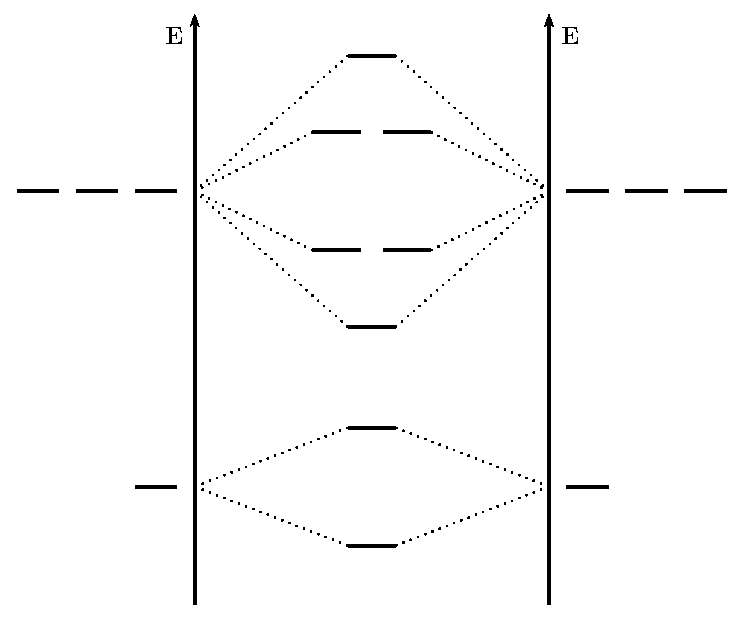
\includegraphics[height=0.4\textheight]{figure/diagOM.eps}\\[0.25cm]
\hline \\[0.25cm]
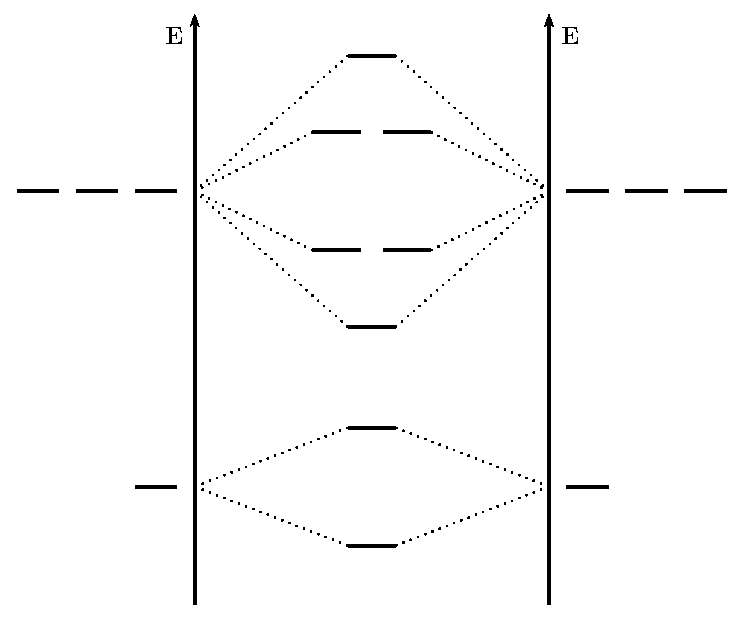
\includegraphics[height=0.4\textheight]{figure/diagOM.eps}\\
\end{tabular}
\end{center}
\end{figure}
\clearpage
%
\begin{figure}[!h]
\begin{center}
\begin{tabular}{c}
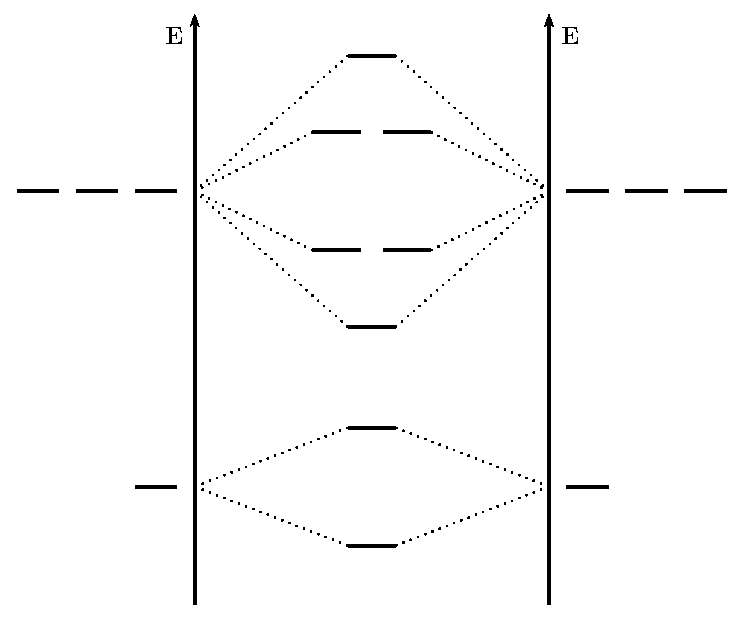
\includegraphics[height=0.4\textheight]{figure/diagOM.eps}\\[0.25cm]
\hline \\[0.25cm]
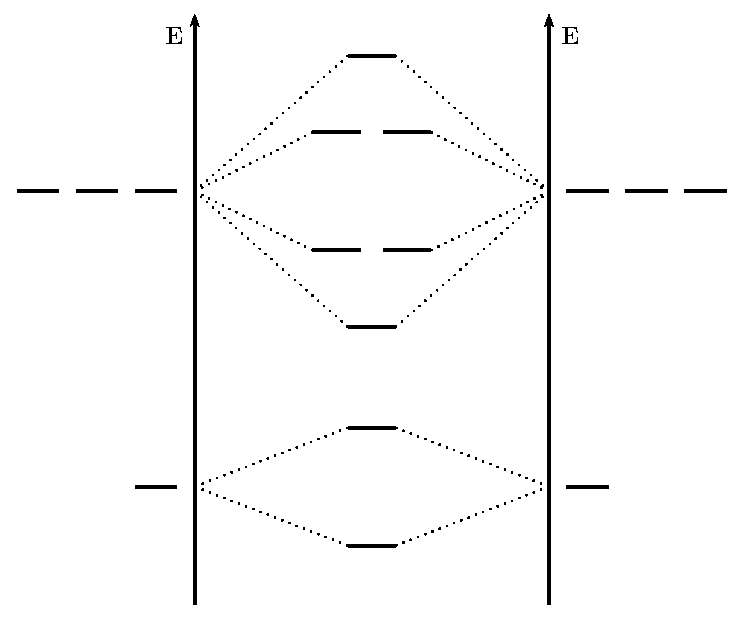
\includegraphics[height=0.4\textheight]{figure/diagOM.eps}\\
\end{tabular}
\end{center}
\end{figure}
\clearpage

\titreTD{\thenumTD}{Mod\`ele ondulatoire}

\begin{center}
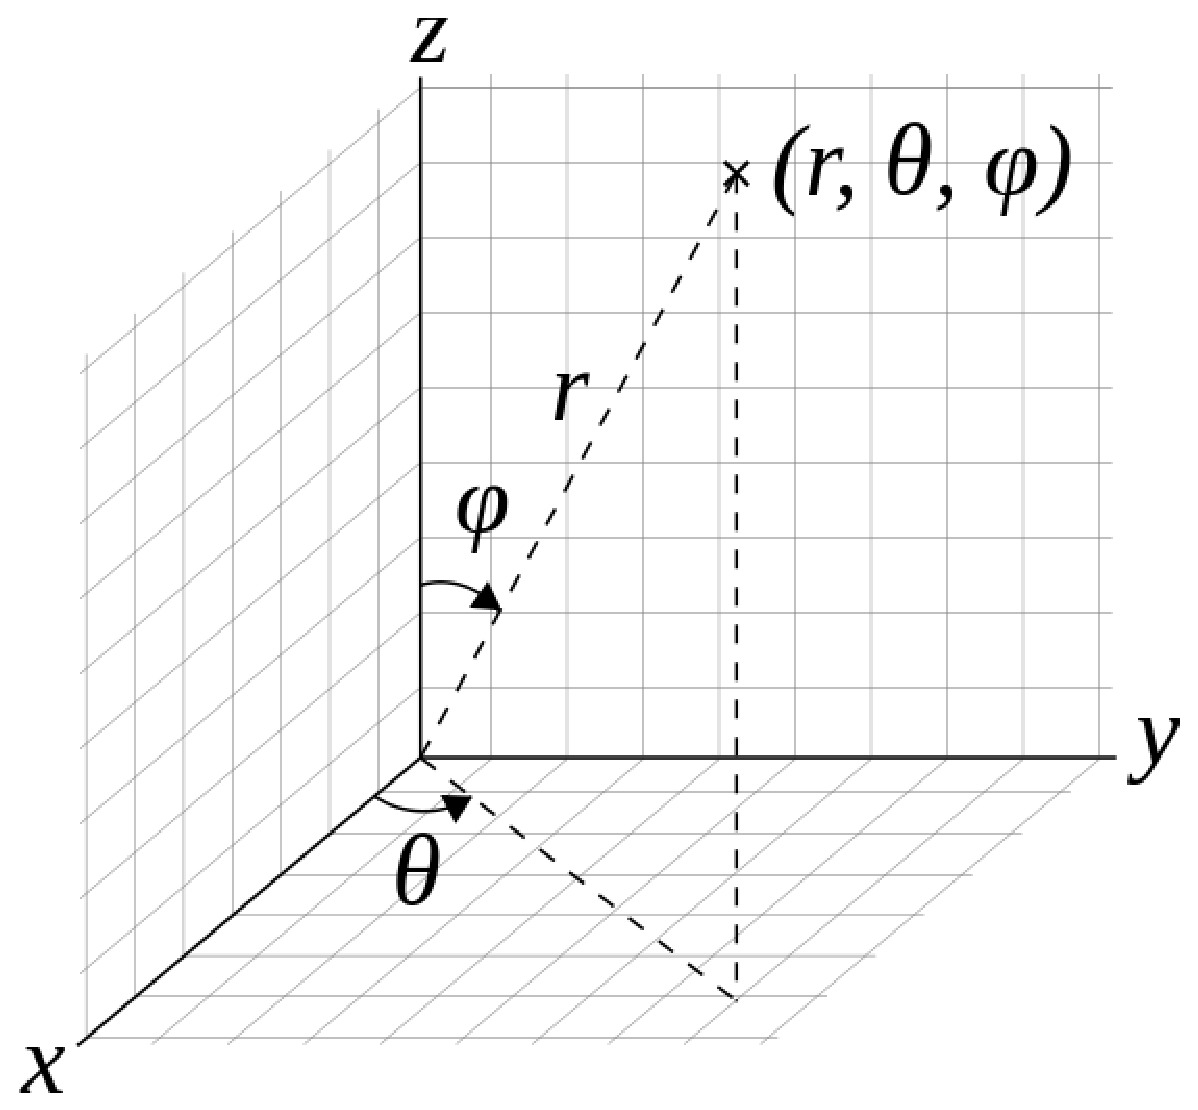
\includegraphics[height=9.5cm]{figure/spheriques.eps}\\
\end{center}

\exo{Fonctions de type ns}

Les trac\'es de la partie radiale des orbitales $1s$, $2s$ et $3s$ de l'atome d'hydrog\`ene 
sont repr\'esent\'es ci-apr\`es.
Tracez de mani\`ere qualitative la densit\'e de probabilit\'e radiale pour les orbitales
$1s$, $2s$ et $3s$. Commentez. 

\begin{center}
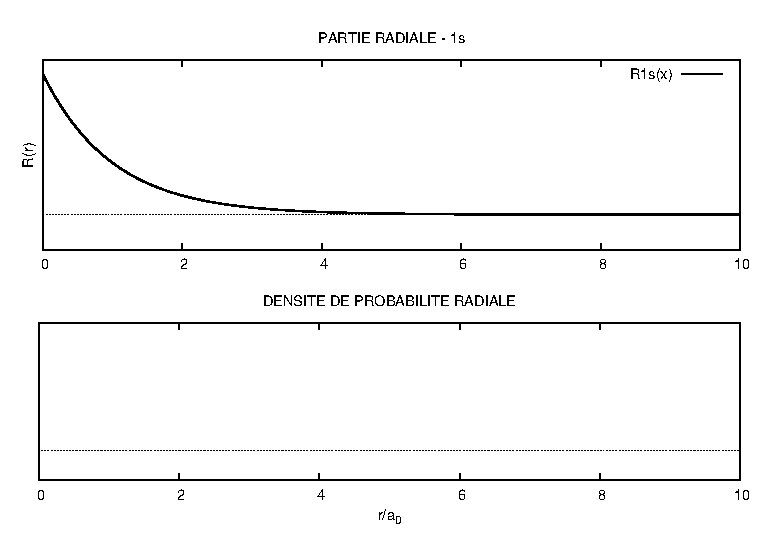
\includegraphics[angle=90,width=0.99\textwidth]{figure/rad1s.eps}
\end{center}

\begin{center}
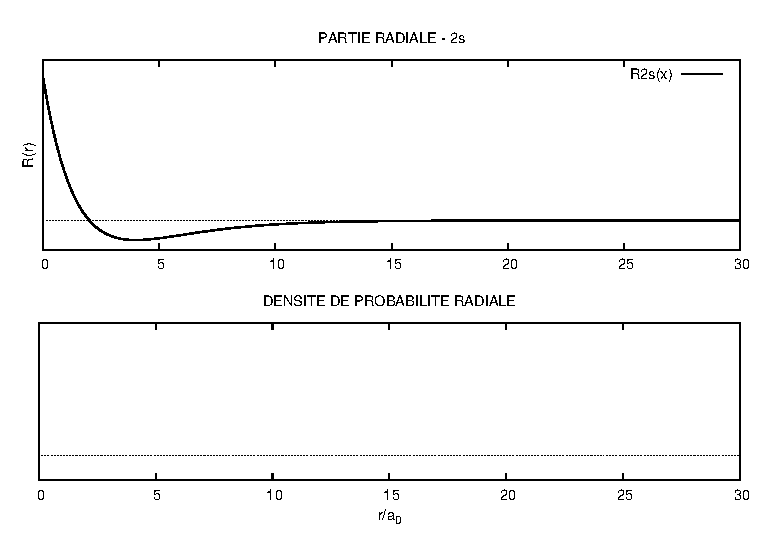
\includegraphics[angle=90,width=0.99\textwidth]{figure/rad2s.eps}
\end{center}

\begin{center}
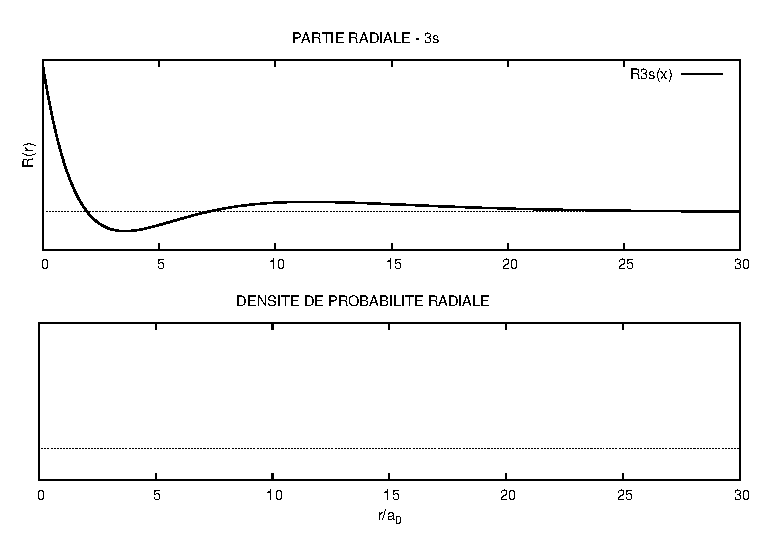
\includegraphics[angle=90,width=0.99\textwidth]{figure/rad3s.eps}
\end{center}

\exo{Mod\`ele de Bohr et mod\`ele quantique}

Dans le mod\`ele de Bohr, l'\'electron est d\'ecrit par des orbites circulaires, 
de rayon $r_n= \frac{n^2}{Z} a_0$ (avec $a_0=0.53$~\AA, $Z$ le num\'ero
atomique et $n$ un entier).
Ce mod\`ele est remplac\'e par le mod\`ele quantique, avec des orbitales \`a la place des orbites. Dans ce dernier
mod\`ele on peut d\'efinir la densit\'e de probabilit\'e radiale. Celle-ci est trac\'ee en Figure~\ref{dens_prop} 
pour l'orbitale 
$1s$ de l'atome d'hydrog\`ene (on a trac\'e en gris\'e la zone o\`u la courbe est proche de son maximum).

\begin{figure}[h]
\begin{center}
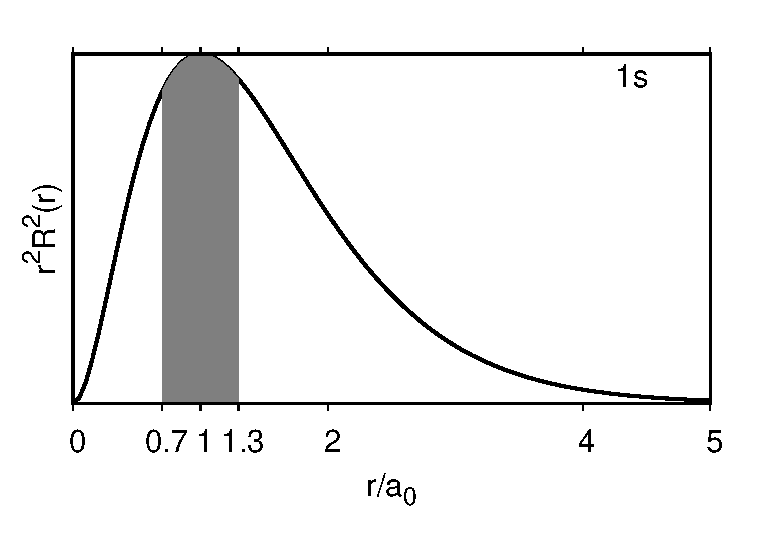
\includegraphics[width=6cm]{figure/area_1s_3.eps}
\caption{Densit\'e de probabilit\'e radiale pour l'orbitale $1s$.}
\label{dens_prop}
\end{center}
\end{figure}

\begin{enumerate}
\item Commentez rapidement cette courbe (position du maximum, tendance à longue distance, valeur au niveau du noyau).
\item Comparez les deux mod\`eles vis-\`a-vis de la trajectoire de l'\'electron autour du noyau. 
\end{enumerate}

%\exo{Normation d'une fonction d'onde $-$ Repr\'esentation graphique}
%
%L'\'etat fondamental de l'atome d'hydrog\`ene est d\'ecrit par la fonction d'onde~:
%
%\[
%%\Psi_{1s}(r,\theta,\varphi)=N.e^{-r/a_0} \qquad \textrm{avec~}N\textrm{~scalaire}
%\begin{array}{rcl}
%\Psi_{1s}(r,\theta,\varphi) &=& R(r) Y(\theta,\varphi) \qquad \text{o\`u}\\[0.3cm]
%R(r)                        &=& N_r e^{-r/a_0}        \\
%Y(\theta,\varphi)           &=& N_{\theta,\varphi} f(\theta,\varphi) \qquad f(\theta,\varphi) = 1\\
%\end{array}
%\]
%avec $N_r$ et $N_{\theta,\varphi}$ scalaires.
%
%\begin{enumerate}[\bf 1)]
%\item Sachant qu'en coordonn\'ees sph\'eriques l'\'el\'ement diff\'erentiel de volume s'\'ecrit
%
%$$
%dV=d\tau=r^2\sin{\theta}dr d\theta d\varphi
%$$
%
%et que l'ensemble de l'espace est d\'ecrit lorsque $r$ varie de $0$ \`a $+\infty$, 
%$\theta$ de $0$ \`a $\pi$ et $\varphi$ de $0$ \`a $2\pi$, \'ecrire l'expression de l'int\'egrale de 
%normalisation.\\
%
%\item \'Ecrire cette int\'egrale sous la forme d'un produit d'une int\'egrale angulaire~:
%\[ 
%N_{\theta,\varphi}^2 \int_0^\infty \int_0^{2\pi} f(\theta,\varphi) \sin{\theta} d\theta d\varphi
%\]
%et d'une int\'egrale radiale que vous det\'erminerez. Normer-les s\'eparemment.
%
%\textbf{On donne~:} $\displaystyle \int_0^{+\infty}r^ne^{-Ar}dr=\frac{n!}{A^{n+1}}$ 
%avec $n$, entier et $A$, r\'eel $> 0$.
%
%\item \'Ecrire la $\Psi_{1s}(r,\theta,\varphi)$ totale. 
%
%\item Rappeler les d\'efinitions de la probabilit\'e de pr\'esence et de la densit\'e 
%de probabilit\'e radiale. Donner l'expression de la densit\'e de probabilit\'e radiale 
%en fonction de la partie radiale $R_{n,l}$ d'une fonction d'onde.
%
%\item Pour la fonction d'onde $\Psi_{1s}$, repr\'esenter graphiquement la courbe donnant, 
%en fonction de $r/a_0$ dans l'intervalle $0 \leq r/a_0 \leq 5$, la densit\'e de 
%probabilit\'e radiale.
%\end{enumerate}


\exo{Repr\'esentation d'orbitale}
L'expression de l'orbitale $1s$ en un point $ M$ de coordonn\'ees  
$(r,\theta,\varphi)$ dans le cas de l'atome d'hydrog\`ene est donn\'ee par~:

$$
\Psi_{1s}(M)=N_s e^{-r/a_0} \ \text{,}
$$

et l'expression de l'orbitale $2p_z$~: 

$$
\Psi_{2p_z}(M)=
N_{p_z}\left(\frac{r}{a_0}\right)e^{-r/2a_0}\cos{\theta} \ .
$$

La densit\'e \'electronique est donn\'ee par~:
$$
D(M)=\Psi^\star(M)\Psi(M)=|\Psi(M)|^2  \ .
$$

\begin{enumerate}

\item Pour l'orbitale $2p_z$, donnez en fonction de $r/a_0$ l'expression de la 
densit\'e \'electronique pour l'ensemble des points $M$ situ\'es sur les axes $Ox$, $Oy$ et $Oz$.

\item Pour l'orbitale $2p_z$, donnez en fonction de $r/a_0$ l'expression de la 
densit\'e \'electronique pour l'ensemble des points $M$ situ\'es que sur l'axe $Oz$. 
Montrez que cette fonction $D(M)$ est maximale pour $r/a_0=2$ 
(tant vers les $z$ positifs, $\theta=0$, que vers les $z$ n\'egatifs, $\theta=180\deg$).

\item Pour quelle valeur de $\theta$ l'orbitale $2p_z$ vaut-elle z\'ero~? Quel est donc le plan nodal~?
Quelle est la densit\'e sur ce plan nodal~?

\item Pour l'orbitale $1s$, donnez en fonction de $r/a_0$ l'expression de la densit\'e 
\'electronique pour l'ensemble des points $M$ situ\'es sur les axes $Ox$, $Oy$ et $Oz$. 
Commentez.
\end{enumerate}

%Expression analytique des parties radiales~:
%
%\[
%\begin{array}{lll} 
%R_{1s}(r)  & = &  2 a_0^{-3/2} e^{-r/a_0}\\[0.3cm]
%R_{2s}(r)  & = &  \displaystyle{\frac{1}{\sqrt{2}} a_0^{-3/2} (1 - \frac{r}{2a_0}) e^{-r/2a_0}}\\[0.3cm]
%R_{3s}(r)  & = &  \displaystyle{\frac{2}{3\sqrt{3}} a_0^{-3/2} (1 - \frac{2r}{3a_0} + \frac{2r^2}{27a_0^2}) e^{-r/3a_0}}\\
%\end{array}
%\] 

\exo{R\'ecapitulatif sur les orbitales atomiques}
Soit un tableau relatif aux fonctions d'onde de l'atome d'hydrog\`ene.

\begin{center}
\begin{tabular}{|l|c|c|c|c|c| c|}\hline
orbitales & $R(r)$ & $Y(\theta,\varphi)$ & $E$ (eV) & $n$ & $l$ &  $m_l$\\\hline
$1s$   &           &                     & & & &\\\hline
$2s$   & \textbf{e}&                     & & & &\\\hline
$2p_x$ &           & \textbf{f}          & & & &\cellcolor{gray} \\\hline
$2p_y$ &           &                     & & & &\cellcolor{gray}\\\hline
$2p_z$ &           &                     & & & &\\\hline
\end{tabular}
\end{center}

On donne dans le d\'esordre les expressions des parties radiales et des parties angulaires norm\'ees s\'epar\'ement~:\\
$$
\textbf{a}=2\left(a_0^{-3/2}\right)e^{-r/a_0} \qquad \qquad
\textbf{b}=\frac{\sqrt{3}}{2\sqrt{\pi}}\sin{\theta}\sin{\varphi} \qquad \qquad
\textbf{c}=\frac{1}{2\sqrt{6}}\left(a_0^{-5/2}\right)r.e^{-r/2a_0}
$$
$$
\textbf{d}=\frac{1}{2\sqrt{\pi}}\qquad
\textbf{e}=\frac{1}{\sqrt{2}}\left(a_0^{-3/2}\right)\left(1-\frac{r}{2a_0}\right)e^{-r/2a_0}\qquad
\textbf{f}=\frac{\sqrt{3}}{2\sqrt{\pi}}\sin{\theta}\cos{\varphi}\qquad
\textbf{g}=\frac{\sqrt{3}}{2\sqrt{\pi}}\cos{\theta}
$$

\begin{enumerate}[\bf 1)]
\item Compl\'etez le tableau ci-dessus en pla\c{c}ant dans la case correspondant \`a chaque fonction d'onde, ($1s$, $2s$, $2p_x$, $2p_y$, $2p_z$) les lettres attribu\'ees aux fonctions radiales et angulaires convenables (\textbf{a}, \textbf{b}, \textbf{c}, \textbf{d}, \textbf{e}, \textbf{f} ou \textbf{g}, ci-dessus).\\

\textbf{Remarque~:} une m\^eme fonction peut intervenir dans diff\'erentes cases~: justifiez.

\item On donne les valeurs des \'energies de ces fonctions d'onde~: $-3,$4~eV et $-13,$6~eV. Placez ces valeurs dans les cases convenables du tableau. Pourquoi n'y a-t-il que deux valeurs~?

\item Compl\'etez le tableau en indiquant les valeurs des trois nombres quantiques orbitaux (ou nombres quantiques d'espace) pour chaque fonction d'onde.\\

\textbf{Remarque~:} pour les fonctions $2p_x$, $2p_y$, $2p_z$, seule $2p_z$ a un nombre $m_l$ déterminé: les fonctions $2p_x$ et $2p_y$ sont des mélanges des orbitales pour lesquelles $m_l=\pm 1$.

\item Indiquez sch\'ematiquement les volumes de plus grande probabilit\'e de pr\'esence pour un \'electron $1s$, $2s$, $2p_x$, $2p_y$ ou $2p_z$, gravitant autour d'un noyau situ\'e au centre d'un rep\`ere orthonorm\'e.
\item Pr\'ecisez pour chaque orbitale :
\begin{enumerate}
\item le signe que prend la fonction d'onde dans les diff\'erentes r\'egions de l'espace~;
\item les surfaces nodales s'il y en a.
%\item les propri\'et\'es directionnelles et \'eventuellement les axes de r\'evolution.
\end{enumerate}
\end{enumerate}


%%--------------------------------------------------------------------
\titreTD{\thenumTD}{Les structures de Lewis}
%--------------------------------------------------------------------

\meth{L'algorithme de Lewis}

Rappeler les \'etapes pour construire une structure de Lewis, exemple du CO$_2$ 
(C central).
\textsl{%
\begin{enumerate}[\bf {Étape} 1]
\item Dessiner le squelette $\sigma$ de la molécule.
\item Compter le nombre total d'électrons de valence, on appelle ce nombre $n_2$.
\item Compléter la structure avec des doublets non liants pour que la règle de l'octet soit
respectée pour chaque atome.
\item Compter le nombre d'électrons dessinés. On appelle ce nombre $n_4$.
\begin{itemize}
\item si $n_4$>$n_2$ supprimer deux doublets non liants portés par deux atomes
adjacents et faire une liaison multiple entre ces atomes.
Repéter le processus jusqu'à ce que $n_4=n_2$.
\item sinon ajouter des doublets non liants sur les atomes hypervalents.
Repéter le processus jusqu'à ce que $n_4=n_2$.
\end{itemize}
\item Déterminer les charges formelles. Si deux charges opposées sont portées par deux atomes adjacents
et que l'un d'eux peut-être hypervalent, supprimer un doublet porté par l'atome chargé négativement
et faire une liaison multiple entre les deux atomes.
Repéter le processus autant que nécessaire.
\end{enumerate}}

\exo{Structure de Lewis de mol\'ecules simples}

Pour chaque atome des compos\'es suivants  (diff\'erents de H), indiquer sa position dans 
le tableau p\'eriodique (p\'eriode et groupe). Compter les \'electrons de valence
et donner la structure de Lewis de chaque compos\'e. 
\'Etablir la charge de chaque atome.
%\'Etablir la charge et le degr\'e d'oxydation de chaque atome.

\begin{center}
\begin{tabular}{lll}
\hline                                           
H$_2$O      & HCN      & PCl$_3$                   \\
CH$_4$      & CH$_3$OH & CH$_3$CH$_3$              \\
NH$_3$      & HBr      & H$_2$S                    \\
NH$_2$OH    & SiH$_4$  & HCl                       \\
NF$_3$      & PH$_3$   & BH$_3$                    \\
\hline
\end{tabular}
\end{center}

\exo{Structures de Lewis et p\'eriode 3}

%Pour les syst\`emes suivants, \'etablir les structures de Lewis, la charge et le degr\'e
%d'oxydation de chaque atome. Quel est la particularit\'e des \'el\'ements P, Cl et S dans ces compos\'es~?
Pour les syst\`emes suivants, \'etablir les structures de Lewis et la charge de chaque atome.
Quel est la particularit\'e des \'el\'ements P, Cl et S dans ces compos\'es~?

{\small \textit{Pour construire le squelette de la mol\'ecule~: l'atome central est en gras et les atomes d'hydrog\`ene 
sont connect\'es aux atomes d'oxyg\`ene.}}

\vspace{0.5cm}

%\centerline{H$_3$\textbf{P}O$_4$, H$_3$\textbf{P}O$_2$, H$_2$\textbf{S}O$_4$, H\textbf{Cl}O, H\textbf{Cl}O$_4$.}
\centerline{H$_3$\textbf{P}O$_4$, H$_2$\textbf{S}O$_4$, H\textbf{Cl}O$_4$.}

\exo{Structures de Lewis d'ions}

Pour les syst\`emes suivants, \'etablir les structures de Lewis et la charge de chaque atome.

\centerline{PF$_4^+$, CH$_3^+$, CH$_3^-$, NO$_2^-$}

%\exo{Structures de Lewis \'equivalentes} 
%
%Plusieurs structures de Lewis sont envisageables pour les mol\'ecules suivantes. 
%Les \'etablir pour chaque mol\'ecule. 
%
%\vspace{0.5cm}
%
%\centerline{NO$_2^-$, HNO$_3$, SO$_4^{2-}$, SO$_3$, HCO$_3^-$, CO$_3^{2-}$, ClO$_4^-$, O$_3$.}
%


%\cleardoublepage

\pagestyle{empty}
\begin{center}
\vspace*{10cm}
\textbf{\Huge Annexe}
\end{center}

\clearpage

\vspace*{10cm}

{\large
\begin{center}
\begin{tabular}{l|ccccc}
\multicolumn{6}{l}{\bf Constantes de Slater}\\
\hline
      & 1s   &  2s2p  &   3s3p &   3d  &  4s4p \\
\hline
1s    & 0,30 &        &        &       &       \\
2s2p  & 0,85 &  0,35  &        &       &       \\
3s3p  & 1    &  0,85  &   0,35 &       &       \\
3d    & 1    &  1     &   1    &   0,35&       \\
4s4p  & 1    &  1     &   0,85 &   0,85&   0,35\\
\hline
\end{tabular}
\end{center}
}

%%\begin{appendix}
%\part{Exercices suppl\'ementaires}
%\include{annexe1}
%\include{annexe4}
%%\end{appendix}




%%\begin{appendix}
%\part{Exercices suppl\'ementaires}
%\include{annexe1}
%\include{annexe4}
%%\end{appendix}

\end{document}
